
\documentclass{article}

\usepackage{graphicx}
\usepackage{changepage}
\usepackage{textgreek}
\usepackage{amsmath}
\usepackage[margin=0.8in]{geometry}
\usepackage{amsmath}
\usepackage{booktabs}
\usepackage{array}
\usepackage{float}
\usepackage{natbib}
\usepackage{placeins}
\usepackage{graphicx}
\usepackage{subcaption}
\graphicspath{ {./images/} }

\begin{document}

\begin{titlepage}
   \vspace*{\stretch{1.0}}
   \begin{center}
      \Large\textbf{Munkacím}\\
       \medskip
      \large\textit{Kotró Balázs}\\
      \medskip
      \large{Draft version}
   \end{center}
   \vspace*{\stretch{2.0}}
\end{titlepage}




\begin{abstract}\rm
\begin{adjustwidth}{0.1cm}{0.1cm}{\itshape\textbf{Abstract:}} 
This paper is examining the linkages between the whole tenor structure of the yield curves of 12 sovereigns from all over the globe. The curves got decomposed to level, slope and curvature factors by the Nelson Siegel model. TBC…
\end{adjustwidth}
\end{abstract}

\section{Bevezetés}


The financial and economic crisis during 2008–2009 renewed interest in understanding the nature of the connectedness among financial markets \cite{aloui2011global}. The attention first turned towards systems when \cite{may1972will} showed that complexity can actually undermine stability. His analysis proves that networks with a larger number of interactions were less stable. The 2008-2009 financial crisis underlined this finding and \cite{haldane2011systemic} argued for the relevance of this insight to the stability of financial systems. Systemic risks within financial systems became the main purpose of investigation by analyzing the presence of co-movement of different assets. To understand how the risk is spread, studies have targeted to understanding the synchronization in varios markets and instruments, especially during the period of the crisis \cite{bisias2012survey}. The banking system was put into the main focus. \cite{acemoglu2015systemic} pointed out that negative shocks affecting sufficiently small financial networks, a densely connected system enhances financial stability, however, beyond a certain point, the opposite phenomenon happens.  \cite{elliott2014financial} showed that integration and diversification within a network has opposite effects. In a small universe cascades can trave among the participants, but as it gets bigger, organizations will have insurance against each other’s failure. With integration growig, dependence on other counterparties grows, but sensitivity on own investments decreases. Besides theoretical studies, empirical articles also captured the connectedness. With econometric models \cite{billio2012econometric} examined the monthly returs of stocks of hedge funds, banks, broker/dealers and the insurance companies, finding that banks play the most important rules of transmitting shocks. \cite{diebold2014network} proved that similar connections can be created based on equity volatility data, chosing seven commercial banks, two investment banks, one credit card company, two mortgagefinance companies and one insurance company.

\section{Irodalmi áttekintés}

\section{Methodology}
\noindent
\subsection{The Nelson and Siegel framework}

Among the statistical models for interest rate, the influential model designed by Diebold-Li [Diebold \& Li, 2006] is widely used in market applications. This model is a dynamic extension of the Nelson-Siegel model ([Nelson \& Siegel, 1987]) for the cross-section fit for the yield curve. The Nelson-Siegel model corresponds to fitting the following equation for the yield curve observed inthe market on a specific date:

\begin{equation}
y_{it}(m_{it})=\beta_{1t}+\beta_{2t}\left ( \frac{1-e^{-\lambda\tau_t}}{\lambda\tau_t} \right )+\beta_{3t}\left ( \frac{1-e^{-\lambda\tau_t}}{\lambda\tau_t} -e^{-\lambda\tau_t}\right )+ \epsilon_{it}
\end{equation}

where \textit{y\textsubscript{it}(m\textsubscript{it})} are the observed rates on a given date \textit{i} and maturity \textit{t}, and \textbeta\textsubscript{1t}, \textbeta\textsubscript{2t}, \textbeta\textsubscript{3t} 
and \texttau\textsubscript{t} are parameters. The Nelson-Siegel model is a parsimonious way of fitting the yield curve while managing to capture a part of the stylized facts in interest rate process, such as the exponential formats present in the yield curves.  The parameters \textbeta\textsubscript{it} have economic interpretations, where textbeta\textsubscript{1t} presents a long-term level interpretation, \textbeta\textsubscript{2t} short-term components, and \textbeta\textsubscript{3t} medium-termcomponents. It may also be interpreted as decompositions of Level, Slope and Curvature of the yield curve, according to the terminology developed by [Litterman \& Scheinkman, 1991]. These components may be used directly in the immunization process of interest rate portfolios. 

The purpose of these models is to allow fitting, and subsequent interpolationsand extrapolations of the yield curve based on a parametric structure, which concurs with othernon-parametric fitting models such as smoothing-splines. Besides the parsimonious estimation,the [Nelson \& Siegel, 1987] model 
has two additional advantages over non-parametric models. The first advantage is that the extrapolation of the curve has a better performance due to the exponential nature of this model.  The second advantage is that the parameters \textbeta\textsubscript{1t}, \textbeta\textsubscript{2t} and \textbeta\textsubscript{3t} have interpretation of level, slope and curvature compatible with the interpretation of three factors proposed by [Litterman \& Scheinkman, 1991], a benchmark in literature. This makes theinterpretation and comparison of the results obtained in the curve fitting easier.The extension formulated by [Diebold \& Li, 2006] renders the [Nelson \& Siegel, 1987] model dynamic (adjusting the several days observed for the yield curve) by means of a procedure in 3 stages:

\begin{itemize}
\item The Nelson-Siegel model (with \texttau fixed, thus making the model linear in the parameters) is fitted by Ordinary Least Squares for each date, estimating the parameters \textbeta\textsubscript{1t}, \textbeta\textsubscript{2t}, \textbeta\textsubscript{3t}.
\item The dynamics of the system is modelled by a vector autoregressive (VAR) model for the parameters \textbeta\textsubscript{1t}, \textbeta\textsubscript{2t} and \textbeta\textsubscript{3t}, estimated in the first stage. 
\item Forecasts for these parameters are made through the VAR model estimated for vectors \textbeta\textsubscript{1t}, \textbeta\textsubscript{2t} and \textbeta\textsubscript{3t}. By substituting the forecasted parameters in Nelson-Siegel model given by equation '1' it is possible to forecast future interest rate curves. % here the Swensson equation is missing
\end{itemize}

According to [Diebold \& Li, 2006], this dynamic formulation has the purpose of capturing the set of existing stylized facts in the term structure of interest rates, such as the fact that while the yield curve is crescent and concave, it may also assume inverted shapes like decreasing curves and slope changes. Other stylized facts captured by [Diebold \& Li, 2006] models are the high persistencein the temporal dynamics (rates with same maturity are highly dependent on the past), and the fact that persistence in the long-term rates is higher than in the short-term rates.

\subsection{The Toda-Yamamoto model}

The Toda–Yamamoto procedure begins from the following premise: The implementation
of the classic Granger Causality test from a VAR (Vector AutoRegressive) model can lead to non-stationarity problems in the series, as it is necessary to confirm the type of existing
cointegration. The authors of ... point out that the “conventional” Wald test produces
integrated or cointegrated causal VAR models, which would inevitably lead to obtaining spurious
Granger causality relationships. However, the Toda–Yamamoto procedure drastically avoids
this handicap by developing a Modified Wald test (MWALD) for restrictions on the parameters
of a VAR \textit{(p)} model. This test is generated on a \textchi\textsubscript{p}  distribution, with \textit{p = p + d\textsubscript{max}} (or number of
time lags). In Wolfe-Rufael’s words, the fundamental idea underlying this procedure is to
“artificially augment the correct VAR order, \textit{p}, by the maximal order of integration, say \textit{d\textsubscript{max}}. Once this
is done, a \textit{(p + d\textsubscript{max})}-th order of VAR is estimated and the coefficients of the last lagged dmax vector are
ignored”. The resulting VAR  \textit{(p + d\textsubscript{max})} model is formulated in Equations (3) and (4):

\begin{equation}
Y_t=\alpha_0+\sum_{i=1}^{k} \delta_{1i} Y_{t-i}+\sum_{j=k+1}^{d_{max}} \alpha_{1j} Y_{t-j}+\sum_{j=1}^{k} \theta_{1j} X_{t-j} +\sum_{j=k+1}^{d_{max}} \beta_{1j} X_{t-j}+\omega_{1t} \
\end{equation}

\begin{equation}
X_t=\alpha_1+\sum_{i=1}^{k} \delta_{2i} Y_{t-i}+\sum_{j=k+1}^{d_{max}} \alpha_{2j} Y_{t-j}+\sum_{j=1}^{k} \theta_{2j} X_{t-j} +\sum_{j=k+1}^{d_{max}} \beta_{2j} X_{t-j}+\omega_{2t} \
\end{equation}



where \textomega\textsubscript{1t} and \textomega\textsubscript{2t} are the VAR error terms and d\textsubscript{max} is the maximum order of integration, according to
the original specification of the Toda–Yamamoto procedure. Therefore, in Equation (3), causality
in the sense of Granger between \textit{X} and \textit{Y} will be detected, provided that \textdelta\textsubscript{1i}  $\neq$ 0 for every \textit{i}, and, on an
identical basis, Equation (4) will imply causality in the sense of Granger between \textit{X} and \textit{Y} , if \textdelta\textsubscript{2i}  $\neq$ 0 for every \textit{i}.

Once the VAR \textit{(p + d\textsubscript{max})}  model is obtained, the implementation of the Toda–Yamamoto procedure in practice requires the realization of three differentiated steps: 

\begin{itemize}
\item Testing each time-series to conclude the maximum order of integration d\textsubscript{max} of
the variables by using, individually or jointly, the following tests: ADF (Augmented Dickey–Fuller), KPSS (Kwiatkowski–Phillips–Schmidt–Shin), and/or PPE (Phillips-Perron). 

\item Next, the optimal lag length (\textit{p}) should be obtained based on the criteria: AIC (Akaike Information Criterion), FPE (Akaike’s Final Prediction Error), SC (Schwartz), HQ (Hannan and Quinn), and LR
(Likelihood-Ratio), seeking, as much as possible, an optimal length supported by the maximum degree of unanimity between criteria. 

\item Finally, the Granger causality test between the variables \textit{X} and \textit{Y} (in both directions) is properly performed by considering that the rejection of the null hypothesis implies
the existence of causality in the sense of Granger according to the Toda–Yamamoto procedure and that a reciprocal rejection would indicate a bilateral causal relationship between the analyzed variables.
\end{itemize}

\subsection{Multilayer causality based network}

We denote the proposed mulitilayer causality based networks as $\overline{\mbox{\textOmega}}$ = \textit{\{G\textsuperscript{[1]},G\textsuperscript{[2]},...G\textsuperscript{[L]}\}}
with \textit{L} layers and \textit{N} nodes, where \textit{\{G\textsuperscript{[\textalpha]}\} = G(V, A\textsuperscript{[\textalpha]})} is layer \textit{\textalpha{}} of multilayer causality based networks, \textit{V = \{1,2,...,N\}}
is the set of nodes, and  \textit{A\textsuperscript{[\textalpha]}} is the set of edges of layer \textit{\textalpha}. On each layer, nodes represent a yield curve factor, and a directed edge indicates that there is a corresponding causality effect from the staring node to the terminal one. In our case \textit{L}=3, and we assume that the first layer, the second layer and the third layer corresponds to level, slope and curvature layers, respectively.
For any two factors \textit{i,j $\in$ V}, we draw a direct edge from \textit{i} to \textit{j} on the first (second, third) layer, if node \textit{i} has a level (slope, curvature) causing effect on node \textit{j}.
\textit{A\textsuperscript{[\textalpha]}}=\textit{\{{a$^{\text{[\textalpha]}}_{\text{ij}}$\}\textsubscript{$N\times N$}}} is a directed binary connection matrix for all pairs of nodes \textit{i} and \textit{j} olayer \textit{\textalpha{}}, where the element \textit{a$^{\text{[\textalpha]}}_{\text{ij}}$} in the matrix \textit{A\textsuperscript{[\textalpha]}} is defined as

\begin{equation}
  \alpha_{ij} =
    \begin{cases}
      1 & \text{if $i$ $\neq$ $j$ and $i$ has a correspopnding causality effect on $j$ layer \textalpha{}}\\
      0 & \text{otherwise}
    \end{cases}       
\end{equation}

Thus, multilayer information spillover networks are simplified to a 3 dimensional $N\times N$ adjacency matrix by mathematical notation. Considering the unpredictability of the financial system and the dynamic changes of interconnectedness amon the yield curve nodes, we build time-varying multilayer causality based networks using rolling window analysis. TBC...




\section{Data}
We obtain daily sovereign yield data from Bloomberg for twelve advanced countries. Our scope is covering multiple reginos of the globe, therefore we picked countries from differenct continents. Eventually four regions were identified with three sovereign each: Pacific (Australia, China, Japan); Americas (Canada, Mexico, United States of America), Eurozone (France, Germany, Italy) and the Non-Eurozone (Great Britain, Norway, Switzerland). We are denoting them with the three letter country codes obtained from The World Bank. Therse are AUS, CHN, JPN, CAD, MEX, USA, FRA, DEU, ITA, GBR, NOR, CHE respectively. The empirical analysis focuses on whole tenor structure of government yields with fifteen maturities: 3, 6, 12, 24, 36, 48, 60, 72, 84, 96, 120, 180, 240 and 360 months.
Below is the table consists of the corresponding Bloomberg iddentification codes for the sovereigns.

\begin{table}[ht]
\caption{This is the eaxemple table}% title of Table
\fontsize{10}{10}\selectfont
\centering % used for centering table
\begin{tabular}{l l}% centered columns (4 columns)
\hline\hline   \\ [-1.5ex]               %inserts double horizontal lines
%Case & Method\#1 & Method\#2 & Method\#3 & test \\  [0.5ex]
Series ID & Description\\ [0.5ex] % inserts table %heading

\hline       \\ [-1.5ex]           % inserts single horizontal line

AUS	 & Australia Sovereign (IYC 1)	\\
CHN & China (IYC 299)  Zero Coupon Yields	\\
JPN	 & Japan Sovereign (IYC 18) Zero Coupon Yields	\\
CAN & Canada Sovereign (IYC 7) Zero Coupon Yields	\\
MEX	 & Mexico (IYC 251)  Zero Coupon Yields	\\
USA & Treasury Actives (IYC 25) Zero Coupon Yields	\\
FRA	 & France Sovereign (IYC 14) Zero Coupon Yields	\\
GER	 & German Sovereign (IYC 16) Zero Coupon Yields	\\
ITA & Italy Sovereign (IYC 40) Zero Coupon Yields	\\
GBR & United Kingdom (IYC 22) Zero Coupon Yields	\\
NOR & Norway (IYC 78)  Zero Coupon Yields	\\
CHE	 & Switzerland (IYC 82)  Zero Coupon Yields	\\
\hline%inserts single line
\end{tabular}
\label{table:nonlin}% is used to refer this table in the text
\end{table}

The data spawns from July 1 2004 to December 31 2019 which means 4045 data points alltogether. This unusual choose of starting date is the reason of this being the first observation date for the Chinese yield curve. Additionally we were not keen on examining the recent consequences of the Covid 19 outbreak thus we ended our analysis period at the end of 2019. 

The sovereign bond yields of the mentioned sovereigns are denominated in local currency terms. Local currency debt indicates divergent interest rate cycles of the economy. The local currency bonds reflect the domestic monetary and economic policy stance. Thus the co-movement of local currency bond yields reveals the convergence of monetary policy and business cycles. Moreover the local currency denominated debt possesses greater liquidity and better credit quality compared to the USD dominated debt. The input data used in this study reflects extracted latent factors of each country using their zero coupon yield rates that mirror their domestic term structure. Table 1 presents the descriptive statistics of bond yields at representative maturities for countries considered in the study. The yield curves are upward sloping for all sample countries (CHECK CRYSIS).

The Dynamic Nelson Siegel model was used to extract the latent factors, Level, Slope and Curvature, for each country separately, following Diebold et al. (2006) and Diebold et al. (2008). The level representing long-term interest rates indicates the expected inflation in the long run; the slope representing short-term interest rates reflects the reaction of monetary policy to the cyclical state of the economy; the curvature implies medium-term interest rates (Aguiar-Conraria et al., 2012). 

%-----------------------------------------------------------------------------------teststat table1
%--------------------------------------------------------------------------------------------------------------------------------------------------

\bigskip

Table 2 presents the descriptive statistics of the estimated latent level, slope and curvature factors. The average level factor was positive for all of the countries and was highest for Mexico and lowest for Japan. The average slope showed the typical pattern of ascending yield curves (negative values) (Aguiar-Conraria et al., 2012). The slope is interpreted as the difference between short-term interest rates (3 months), and the long-term interest rates (120 months 360?). Slope was negative for all of the countries, indicating that long-term rates were higher than the short-term rates. The average slope was highest (in absoluter terms) in the US (-3.427) and lowest (in absoluter terms) in Australia (-0.898). The positive values for the slope indicate brief episodes associated with restrictive monetary policies.
The curvature also takes negative values for all counties. It was highest in France and lowest in China. 

The raw series of level, slope and curvature were tested for normality using Jarque-Bera test. All 36 values failed to meet the criterion, thus we can state that neither time series follow normal distribution. 
Additionally the factor values were tested fot unit roots using the Augmented Dickey-Fuller (ADF) and Kwiatkowski-Phillips-Schmidt-Shin (KPSS) tests. China curvature and Japan slope found to be stationary (according to ADF) on standard 95\% confidence level. Differentiating the remaining time series became stationary according to both unit root tests.

Undiferentiated time series were tested for cointegration with pairwise Engle Granger test. Table 4 consists of the ratio of the cointegrated and non-cointegrated time series grouuped by the factors. Taken with self results are more that 70\%, additionally Curvature - Slope and Slope-Curvature pairs exceeds this level too. These results indicate the need of the Toda-Yamamoto approach.




%-----------------------------------------------------------------------------------teststat table2-------------------------------------------------
\begin{table}[H]
\caption{Descriptive statistics of the Diebold-Li factors}% title of Table
\fontsize{10}{10}\selectfont
\centering % used for centering table
\begin{tabular}{l c c c c c c}% centered columns (4 columns)
\hline\hline   \\ [-1.5ex]               %inserts double horizontal lines
%Case & Method\#1 & Method\#2 & Method\#3 & test \\  [0.5ex]
Factor & Mean & Std. Dev & Minimum & Maximum & Jarque-Bera t-statistics  & P values \\ [0.5ex] % inserts table %heading

\hline       \\ [-1.5ex]           % inserts single horizontal line

\textit{Germany}	&		&		&		&		&		&		\\
Level	&	2.915	&	1.535	&	-0.343	&	5.413	&	347.041	&	0	\\
Slope	&	-1.856	&	1.062	&	-4.544	&	0.140	&	210.098	&	0	\\
\medskip													
Curvature	&	-3.723	&	1.720	&	-7.147	&	0.732	&	234.599	&	0	\\
\textit{Italy}	&		&		&		&		&		&		\\
Level	&	4.784	&	1.292	&	1.980	&	7.998	&	106.101	&	0	\\
Slope	&	-3.427	&	1.570	&	-7.009	&	-0.435	&	183.385	&	0	\\
\medskip													
Curvature	&	-4.251	&	2.236	&	-8.604	&	4.752	&	194.464	&	0	\\
\textit{France}	&		&		&		&		&		&		\\
Level	&	3.391	&	1.367	&	0.263	&	5.484	&	417.881	&	0	\\
Slope	&	-2.237	&	1.191	&	-4.731	&	0.016	&	162.987	&	0	\\
\medskip													
Curvature	&	-4.294	&	1.956	&	-7.820	&	1.073	&	210.076	&	0	\\
\textit{USA}	&		&		&		&		&		&		\\
Level	&	3.957	&	0.988	&	1.881	&	5.867	&	323.945	&	0	\\
Slope	&	-2.408	&	1.550	&	-5.519	&	0.710	&	139.147	&	0	\\
\medskip													
Curvature	&	-3.633	&	2.498	&	-9.577	&	0.723	&	228.960	&	0	\\
\textit{Canada}	&		&		&		&		&		&		\\
Level	&	3.431	&	1.102	&	1.232	&	5.897	&	274.286	&	0	\\
Slope	&	-1.726	&	1.228	&	-4.839	&	0.583	&	251.083	&	0	\\
\medskip													
Curvature	&	-2.493	&	1.627	&	-6.257	&	1.307	&	206.333	&	0	\\
\textit{Mexico}	&		&		&		&		&		&		\\
Level	&	8.579	&	1.282	&	5.550	&	13.413	&	834.740	&	0	\\
Slope	&	-2.356	&	1.825	&	-6.135	&	0.674	&	340.695	&	0	\\
\medskip													
Curvature	&	-4.157	&	2.852	&	-14.835	&	0.489	&	321.622	&	0	\\
\textit{Japan}	&		&		&		&		&		&		\\
Level	&	1.703	&	0.828	&	-0.018	&	3.256	&	406.313	&	0	\\
Slope	&	-1.280	&	0.625	&	-2.827	&	-0.019	&	155.924	&	0	\\
\medskip													
Curvature	&	-3.694	&	1.283	&	-6.033	&	-0.874	&	278.292	&	0	\\
\textit{China}	&		&		&		&		&		&		\\
Level	&	4.024	&	0.616	&	2.704	&	6.523	&	2047.454	&	0	\\
Slope	&	-1.531	&	0.809	&	-3.869	&	1.648	&	275.315	&	0	\\
\medskip													
Curvature	&	-1.243	&	0.924	&	-5.198	&	1.259	&	1128.360	&	0	\\
\textit{Australia}	&		&		&		&		&		&		\\
Level	&	4.629	&	1.230	&	1.398	&	6.773	&	262.680	&	0	\\
Slope	&	-0.898	&	0.980	&	-3.868	&	1.003	&	105.808	&	0	\\
\medskip													
Curvature	&	-2.081	&	1.839	&	-6.590	&	2.247	&	296.577	&	0	\\
\textit{Norway}	&		&		&		&		&		&		\\
Level	&	3.215	&	1.124	&	1.024	&	5.228	&	333.917	&	0	\\
Slope	&	-1.223	&	1.072	&	-4.041	&	2.262	&	167.102	&	0	\\
\medskip													
Curvature	&	-1.586	&	1.223	&	-4.681	&	1.726	&	337.556	&	0	\\
\textit{United Kingdom}	&		&		&		&		&		&		\\
Level	&	3.663	&	1.232	&	0.867	&	5.798	&	329.213	&	0	\\
Slope	&	-1.759	&	1.746	&	-5.418	&	1.346	&	211.589	&	0	\\
\medskip													
Curvature	&	-3.329	&	3.021	&	-8.767	&	3.647	&	159.960	&	0	\\
\textit{Switzerland}	&		&		&		&		&		&		\\
Level	&	1.773	&	1.176	&	-0.756	&	3.856	&	289.824	&	0	\\
Slope	&	-1.181	&	0.699	&	-3.323	&	0.909	&	219.716	&	0	\\
Curvature	&	-2.940	&	1.211	&	-7.766	&	0.616	&	543.782	&	0	\\

\hline%inserts single line
\end{tabular}
\label{table:nonlin}% is used to refer this table in the text
\end{table}
%----------------------------------------------------------------------------------------------------------------------------------------------------

\begin{figure}[H]
\caption{Normalized Diebold-Li factor time series}
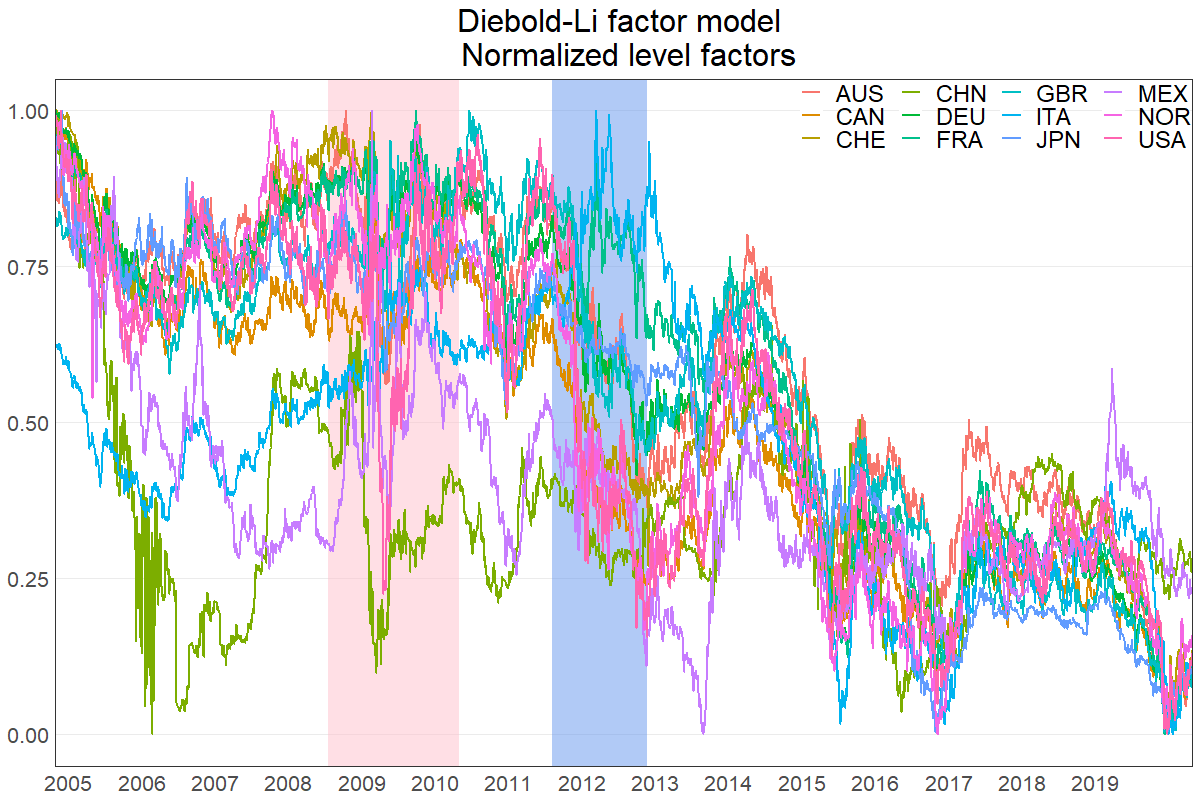
\includegraphics[width=11.5cm]{Normalizedlevel}
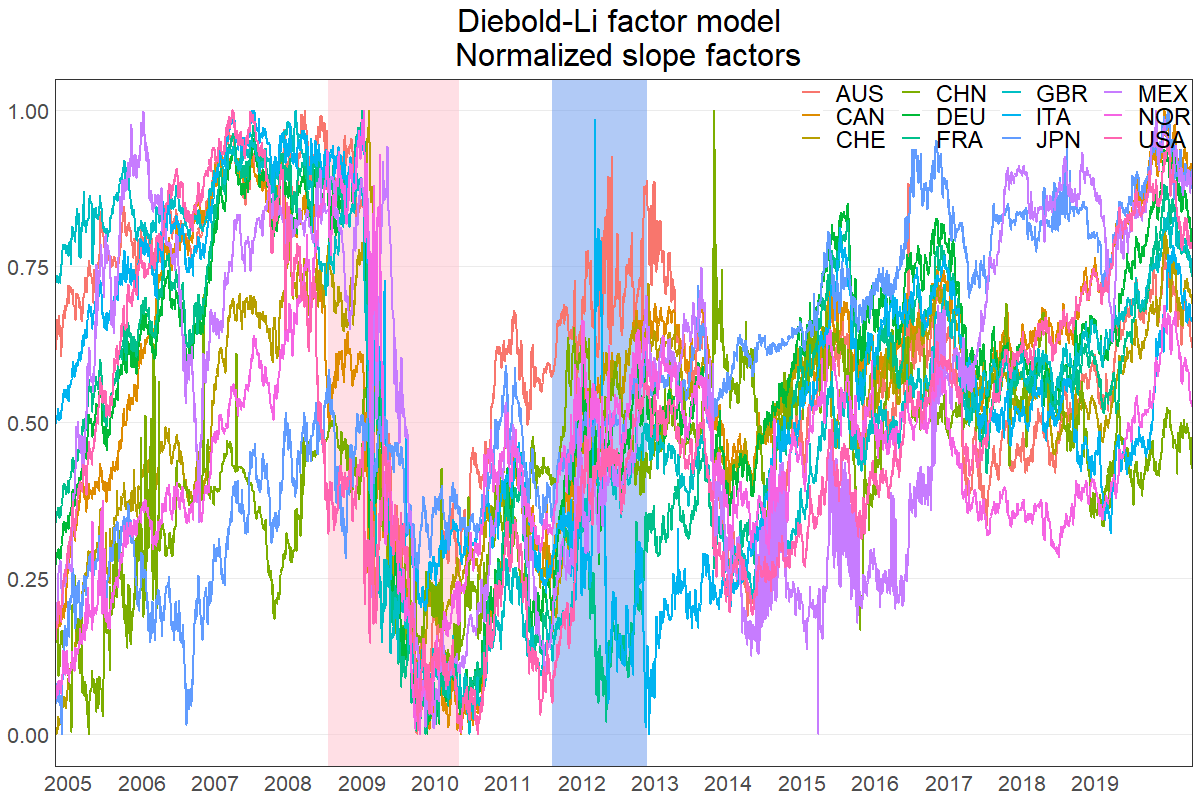
\includegraphics[width=11.5cm]{Normalizedslope}
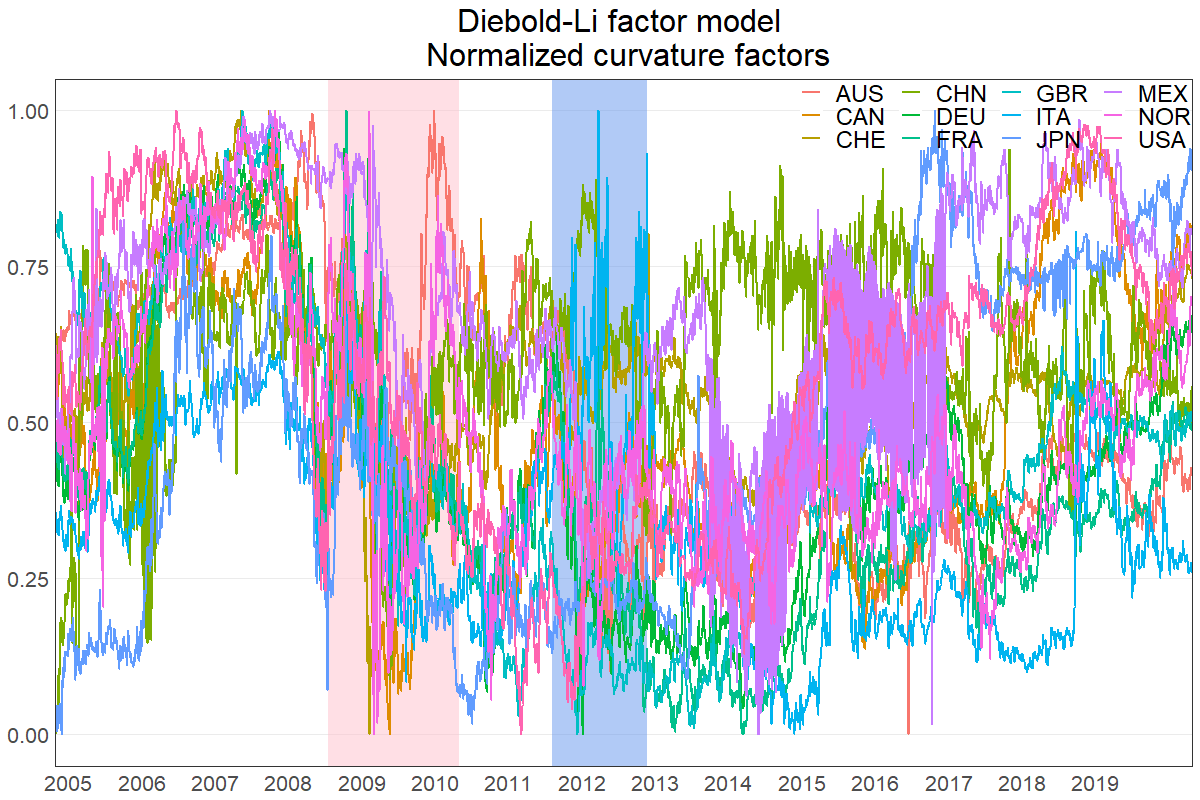
\includegraphics[width=11.5cm]{Normalizedcurvature}
\centering
\end{figure}




%---------------------------------------------------------------------------------ADF Table-------------------------------------------------------
\begin{table}[h]
\caption{ADF} %title of the table
\fontsize{10}{10}\selectfont
\centering% centering table
\begin{tabular}{l cc cc cc cc cc cc}% creating eight columns
\hline\hline \\ [-1.5ex]                         %inserting double-line
%Audio Name&\multicolumn{2}{c}{Sum of Extracted Bits}&\multicolumn{4}{c}{Sum of Extracted Bits} \\ [0.5ex] 

Country	&	\multicolumn{2}{c}{GER}			&	\multicolumn{2}{c}{ITA}			&	\multicolumn{2}{c}{FRA}			&	\multicolumn{2}{c}{US}			&	\multicolumn{2}{c}{CAN}			&	\multicolumn{2}{c}{MXN}			\\[0.5ex] 

 & value &P & value &P& value &P & value &P& value &P & value &P\\

\hline       \\ [-1.5ex] 

Level	&	-2.304	&	0.450	&	-1.461	&	0.806	&	-2.161	&	0.510	&	-3.657	&	0.027	&	-3.060	&	0.129	&	-3.9732	&	0.010	\\
Slope	&	-2.088	&	0.541	&	-2.262	&	0.468	&	-1.641	&	0.730	&	-1.500	&	0.790	&	-1.572	&	0.760	&	-1.881	&	0.629	\\
\medskip
Curvature	&	-2.218	&	0.486	&	-3.592	&	0.033	&	-2.357	&	0.427	&	-1.621	&	0.739	&	-2.351	&	0.430	&	-2.705	&	0.279	\\

\hline\hline   \\ [-1.5ex]    

Country	&	\multicolumn{2}{c}{JPY}			&	\multicolumn{2}{c}{CHN}			&	\multicolumn{2}{c}{AUS}			&	\multicolumn{2}{c}{NEK}			&	\multicolumn{2}{c}{UK}			&	\multicolumn{2}{c}{SWI}			\\

 & value &P & value &P& value &P & value &P& value &P & value &P\\

\hline       \\ [-1.5ex] 

Level	&	-2.972	&	0.167	&	-3.693	&	0.024	&	-2.901	&	0.197	&	-2.630	&	0.312	&	-2.159	&	0.511	&	-2.499	&	0.367	\\
Slope	&	-4.851	&	0.010	&	-3.689	&	0.025	&	-2.303	&	0.450	&	-2.724	&	0.272	&	-0.949	&	0.947	&	-3.135	&	0.099	\\
Curvature	&	-2.032	&	0.565	&	-5.521	&	0.010	&	-2.612	&	0.319	&	-3.695	&	0.024	&	-1.615	&	0.741	&	-3.138	&	0.099	\\

\hline            
\end{tabular}
\label{table:nonlin}% is used to refer this table in the text
\end{table}
%----------------------------------------------------------------------------------------------------------------------------------------------------

%---------------------------------------------------------------------------------KPSS Table-------------------------------------------------------
\begin{table}[h]
\caption{KPSS} %title of the table
\fontsize{10}{10}\selectfont
\centering% centering table
\begin{tabular}{l cc cc cc cc cc cc}% creating eight columns
\hline\hline \\ [-1.5ex]                         %inserting double-line
%Audio Name&\multicolumn{2}{c}{Sum of Extracted Bits}&\multicolumn{4}{c}{Sum of Extracted Bits} \\ [0.5ex] 

Country	&	\multicolumn{2}{c}{GER}			&	\multicolumn{2}{c}{ITA}			&	\multicolumn{2}{c}{FRA}			&	\multicolumn{2}{c}{US}			&	\multicolumn{2}{c}{CAN}			&	\multicolumn{2}{c}{MXN}			\\[0.5ex] 

 & value &P & value &P& value &P & value &P& value &P & value &P\\

\hline       \\ [-1.5ex] 

Level	&	32.897	&	0.010	&	14.577	&	0.010	&	29.872	&	0.010	&	26.849	&	0.010	&	32.182	&	0.010	&	15.235	&	0.010	\\
Slope	&	4.255	&	0.010	&	7.608	&	0.010	&	4.501	&	0.010	&	5.301	&	0.010	&	5.403	&	0.010	&	4.780	&	0.010	\\
\medskip
Curvature	&	8.958	&	0.010	&	10.208	&	0.010	&	15.213	&	0.010	&	7.339	&	0.010	&	4.590	&	0.010	&	4.926	&	0.010	\\


\hline\hline   \\ [-1.5ex]    

Country	&	\multicolumn{2}{c}{JPY}			&	\multicolumn{2}{c}{CHN}			&	\multicolumn{2}{c}{AUS}			&	\multicolumn{2}{c}{NEK}			&	\multicolumn{2}{c}{UK}			&	\multicolumn{2}{c}{SWI}			\\

 & value &P & value &P& value &P & value &P& value &P & value &P\\

\hline       \\ [-1.5ex] 

Level	&	33.938	&	0.010	&	3.546	&	0.010	&	29.172	&	0.010	&	30.064	&	0.010	&	28.697	&	0.010	&	31.964	&	0.010	\\
Slope	&	33.208	&	0.010	&	14.992	&	0.010	&	7.317	&	0.010	&	1.251	&	0.010	&	7.531	&	0.010	&	5.485	&	0.010	\\
\medskip
Curvature	&	15.946	&	0.010	&	2.912	&	0.010	&	24.672	&	0.010	&	11.552	&	0.010	&	13.325	&	0.010	&	5.669	&	0.010	\\


\hline   

\end{tabular}
\label{tab:hresult}
\end{table}
%----------------------------------------------------------------------------------------------------------------------------------------------------

%---------------------------------------------------------------------------------ADF(1) Table-------------------------------------------------------
\begin{table}[h]
\caption{ADF(1)} %title of the table
\fontsize{10}{10}\selectfont
\centering% centering table
\begin{tabular}{l cc cc cc cc cc cc}% creating eight columns
\hline\hline \\ [-1.5ex]                         %inserting double-line
%Audio Name&\multicolumn{2}{c}{Sum of Extracted Bits}&\multicolumn{4}{c}{Sum of Extracted Bits} \\ [0.5ex] 

Country	&	\multicolumn{2}{c}{GER}			&	\multicolumn{2}{c}{ITA}			&	\multicolumn{2}{c}{FRA}			&	\multicolumn{2}{c}{US}			&	\multicolumn{2}{c}{CAN}			&	\multicolumn{2}{c}{MXN}			\\[0.5ex] 

 & value &P & value &P& value &P & value &P& value &P & value &P\\

\hline       \\ [-1.5ex] 

Level	&	-17.051	&	0.010	&	-16.015	&	0.010	&	-15.986	&	0.010	&	-15.788	&	0.010	&	-16.353	&	0.010	&	-16.557	&	0.010	\\
Slope	&	-15.899	&	0.010	&	-14.628	&	0.010	&	-14.593	&	0.010	&	-16.547	&	0.010	&	-16.323	&	0.010	&	-15.194	&	0.010	\\
\medskip
Curvature	&	-18.514	&	0.010	&	-18.671	&	0.010	&	-17.646	&	0.010	&	-17.454	&	0.010	&	-16.016	&	0.010	&	-18.880	&	0.010	\\


\hline\hline   \\ [-1.5ex]    

Country	&	\multicolumn{2}{c}{JPY}			&	\multicolumn{2}{c}{CHN}			&	\multicolumn{2}{c}{AUS}			&	\multicolumn{2}{c}{NEK}			&	\multicolumn{2}{c}{UK}			&	\multicolumn{2}{c}{SWI}			\\

 & value &P & value &P& value &P & value &P& value &P & value &P\\

\hline       \\ [-1.5ex] 

Level	&	-16.555	&	0.010	&	-16.990	&	0.010	&	-15.609	&	0.010	&	-16.432	&	0.010	&	-16.484	&	0.010	&	-15.573	&	0.010	\\
Slope	&		&		&	-18.902	&	0.010	&	-17.872	&	0.010	&	-17.605	&	0.010	&	-16.116	&	0.010	&	-14.598	&	0.010	\\
\medskip
Curvature	&	-17.512	&	0.010	&		&		&	-18.061	&	0.010	&	-17.041	&	0.010	&	-16.451	&	0.010	&	-14.266	&	0.010	\\


\hline            
\end{tabular}
\label{table:nonlin}% is used to refer this table in the text
\end{table}


%----------------------------------------------------------------------------------------------------------------------------------------------------

%---------------------------------------------------------------------------------KPSS(1) Table-------------------------------------------------------
\begin{table}[h]
\caption{KPSS(1)} %title of the table
\fontsize{10}{10}\selectfont
\centering% centering table
\begin{tabular}{l cc cc cc cc cc cc}% creating eight columns
\hline\hline \\ [-1.5ex]                         %inserting double-line
%Audio Name&\multicolumn{2}{c}{Sum of Extracted Bits}&\multicolumn{4}{c}{Sum of Extracted Bits} \\ [0.5ex] 

Country	&	\multicolumn{2}{c}{GER}			&	\multicolumn{2}{c}{ITA}			&	\multicolumn{2}{c}{FRA}			&	\multicolumn{2}{c}{US}			&	\multicolumn{2}{c}{CAN}			&	\multicolumn{2}{c}{MXN}			\\[0.5ex] 

 & value &P & value &P& value &P & value &P& value &P & value &P\\

\hline       \\ [-1.5ex] 

Level	&	0.039	&	0.100	&	0.127	&	0.100	&	0.058	&	0.100	&	0.026	&	0.100	&	0.060	&	0.100	&	0.083	&	0.100	\\
Slope	&	0.083	&	0.100	&	0.073	&	0.100	&	0.118	&	0.100	&	0.158	&	0.100	&	0.171	&	0.100	&	0.091	&	0.100	\\
Curvature	&	0.050	&	0.100	&	0.015	&	0.100	&	0.048	&	0.100	&	0.084	&	0.100	&	0.076	&	0.100	&	0.011	&	0.100	\\


\hline\hline   \\ [-1.5ex]    

Country	&	\multicolumn{2}{c}{JPY}			&	\multicolumn{2}{c}{CHN}			&	\multicolumn{2}{c}{AUS}			&	\multicolumn{2}{c}{NEK}			&	\multicolumn{2}{c}{UK}			&	\multicolumn{2}{c}{SWI}			\\

 & value &P & value &P& value &P & value &P& value &P & value &P\\

\hline       \\ [-1.5ex] 

Level	&	0.026	&	0.100	&	0.156	&	0.100	&	0.049	&	0.100	&	0.036	&	0.100	&	0.073	&	0.100	&	0.042	&	0.100	\\
Slope	&	0.027	&	0.100	&	0.029	&	0.100	&	0.042	&	0.100	&	0.084	&	0.100	&	0.242	&	0.100	&	0.137	&	0.100	\\
Curvature	&	0.059	&	0.100	&	0.045	&	0.100	&	0.037	&	0.100	&	0.030	&	0.100	&	0.160	&	0.100	&	0.045	&	0.100	\\


\hline            
\end{tabular}
\label{table:nonlin}% is used to refer this table in the text
\end{table}
%----------------------------------------------------------------------------------------------------------------------------------------------------

%---------------------------------------------------------------------------------Blocked E-G test Table-------------------------------------------------------
\begin{table}[h]
\caption{Engle-Granger test} %title of the table
\fontsize{10}{10}\selectfont
\centering% centering table
\begin{tabular}{l | ccc}% creating eight columns
\hline\hline \\ [-1.5ex]                         %inserting double-line

	&	Level	&	Slope	&	Curvature	\\
\hline \\ [-1.5ex]  
Level	&	75.694\%	&	44.444\%	&	64.583\%	\\
Slope	&	29.167\%	&	74.306\%	&	71.528\%	\\
Curvature	&	29.167\%	&	78.472\%	&	75.000\%	\\

\hline            
\end{tabular}
\label{table:nonlin}% is used to refer this table in the text
\end{table}

\clearpage 

\section{empirical results}

\begin{figure}[H]
  \begin{subfigure}[t]{.4\textwidth}
    \centering
    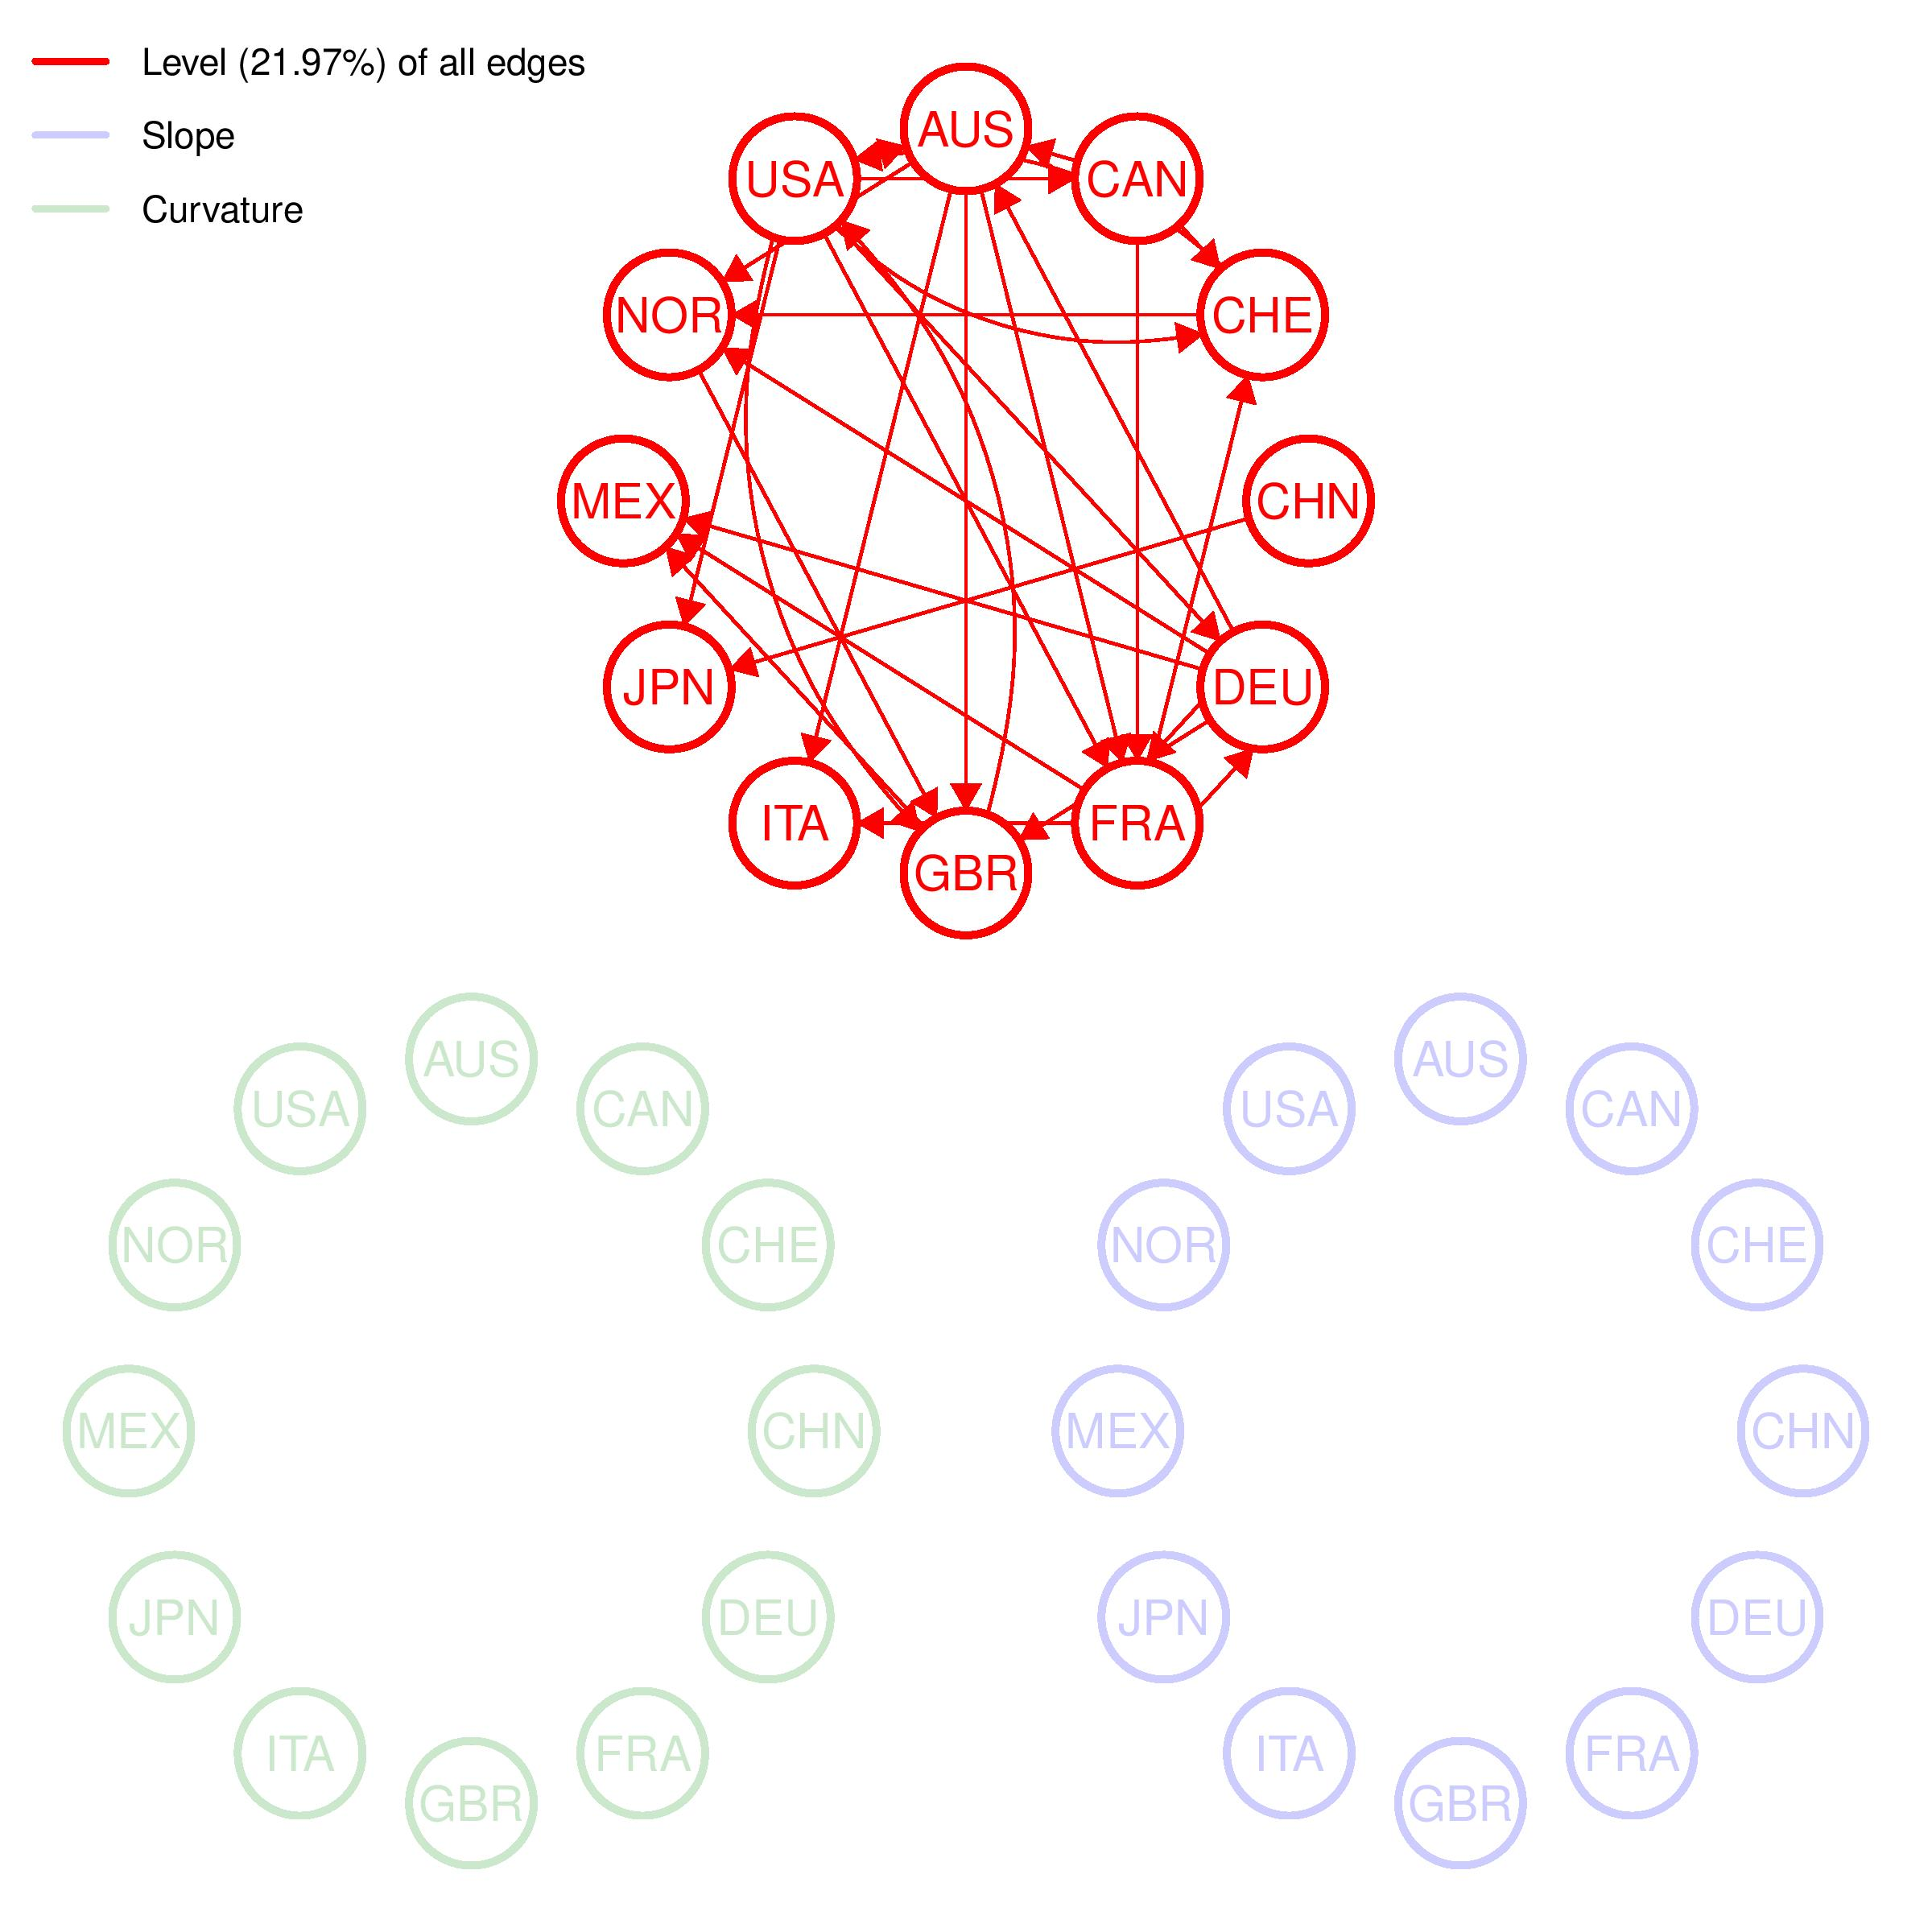
\includegraphics[width=\linewidth]{All_plot_onlylevel2004-07-01_2019-12-31_0.01-page-001}
    \caption{\textbf{Levels only}}
  \end{subfigure}
  \hfill
  \begin{subfigure}[t]{.4\textwidth}
    \centering
    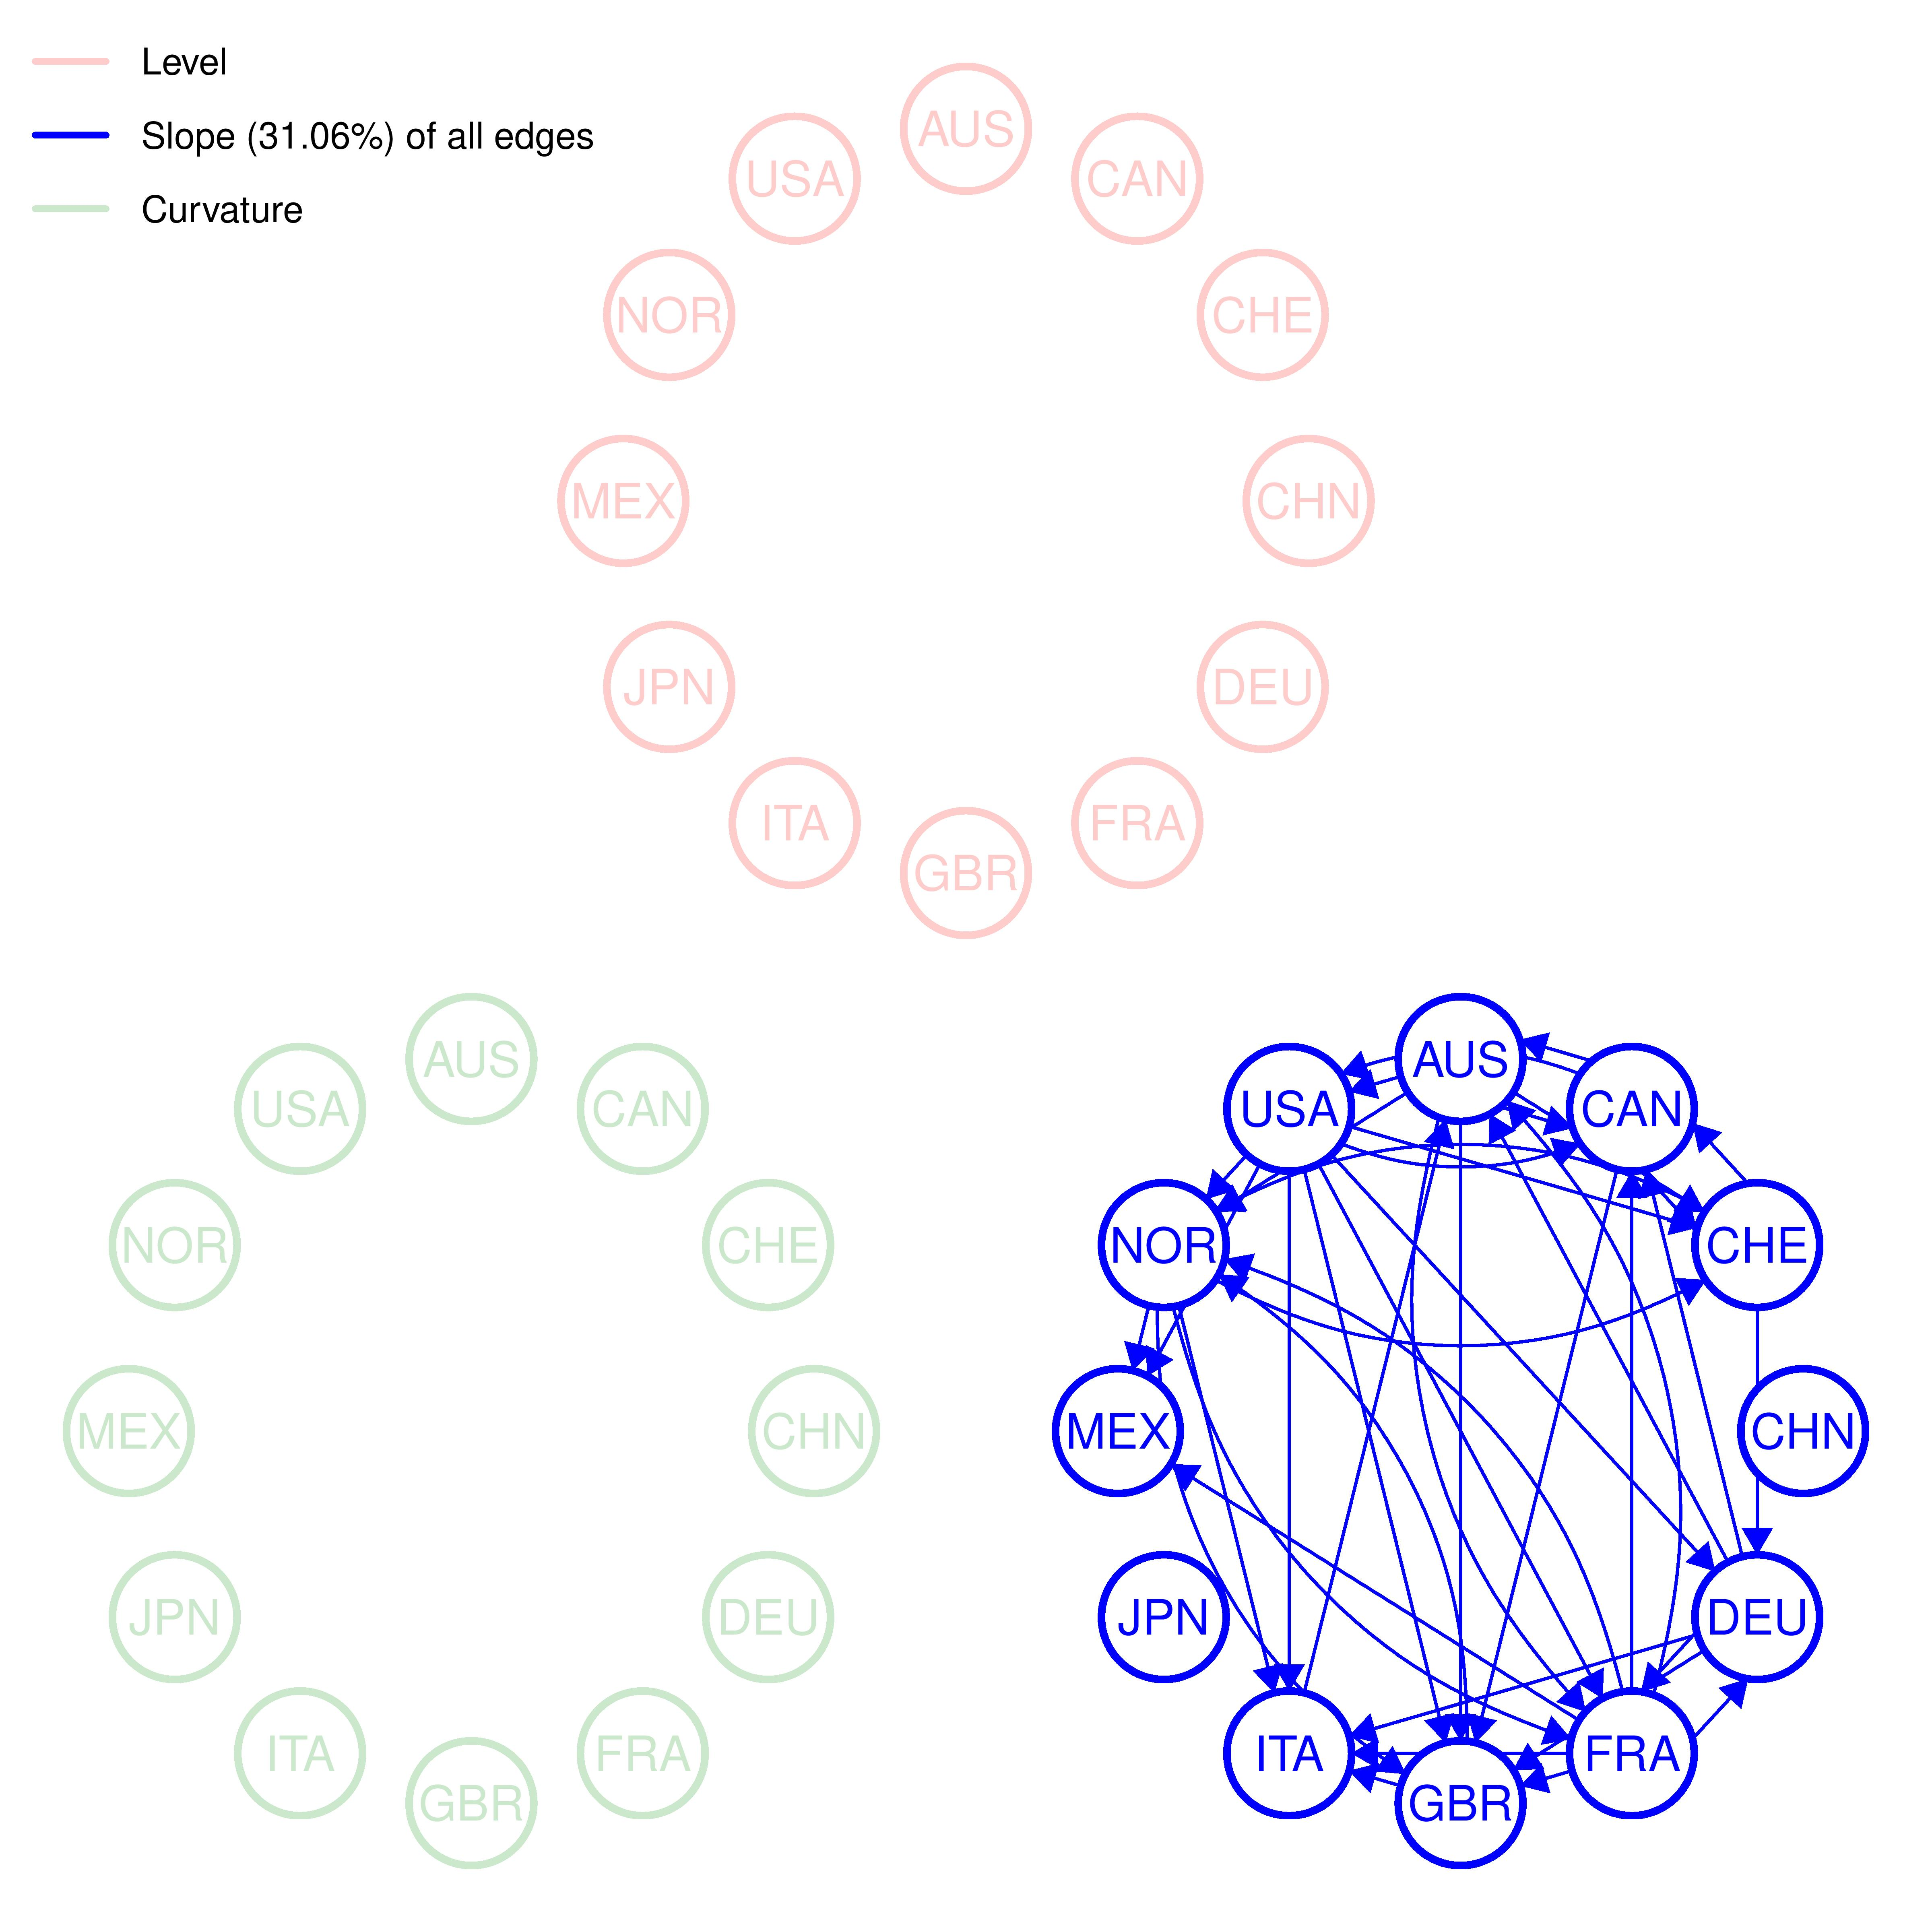
\includegraphics[width=\linewidth]{All_plot_onlyslope_2004-07-01_2019-12-31_0.01-page-001}
    \caption{\textbf{Slopes only}: $A \cap B$: Element liegt in $A$ \textbf{und} in $B$.}
  \end{subfigure}

  \medskip

  \begin{subfigure}[t]{.4\textwidth}
    \centering
    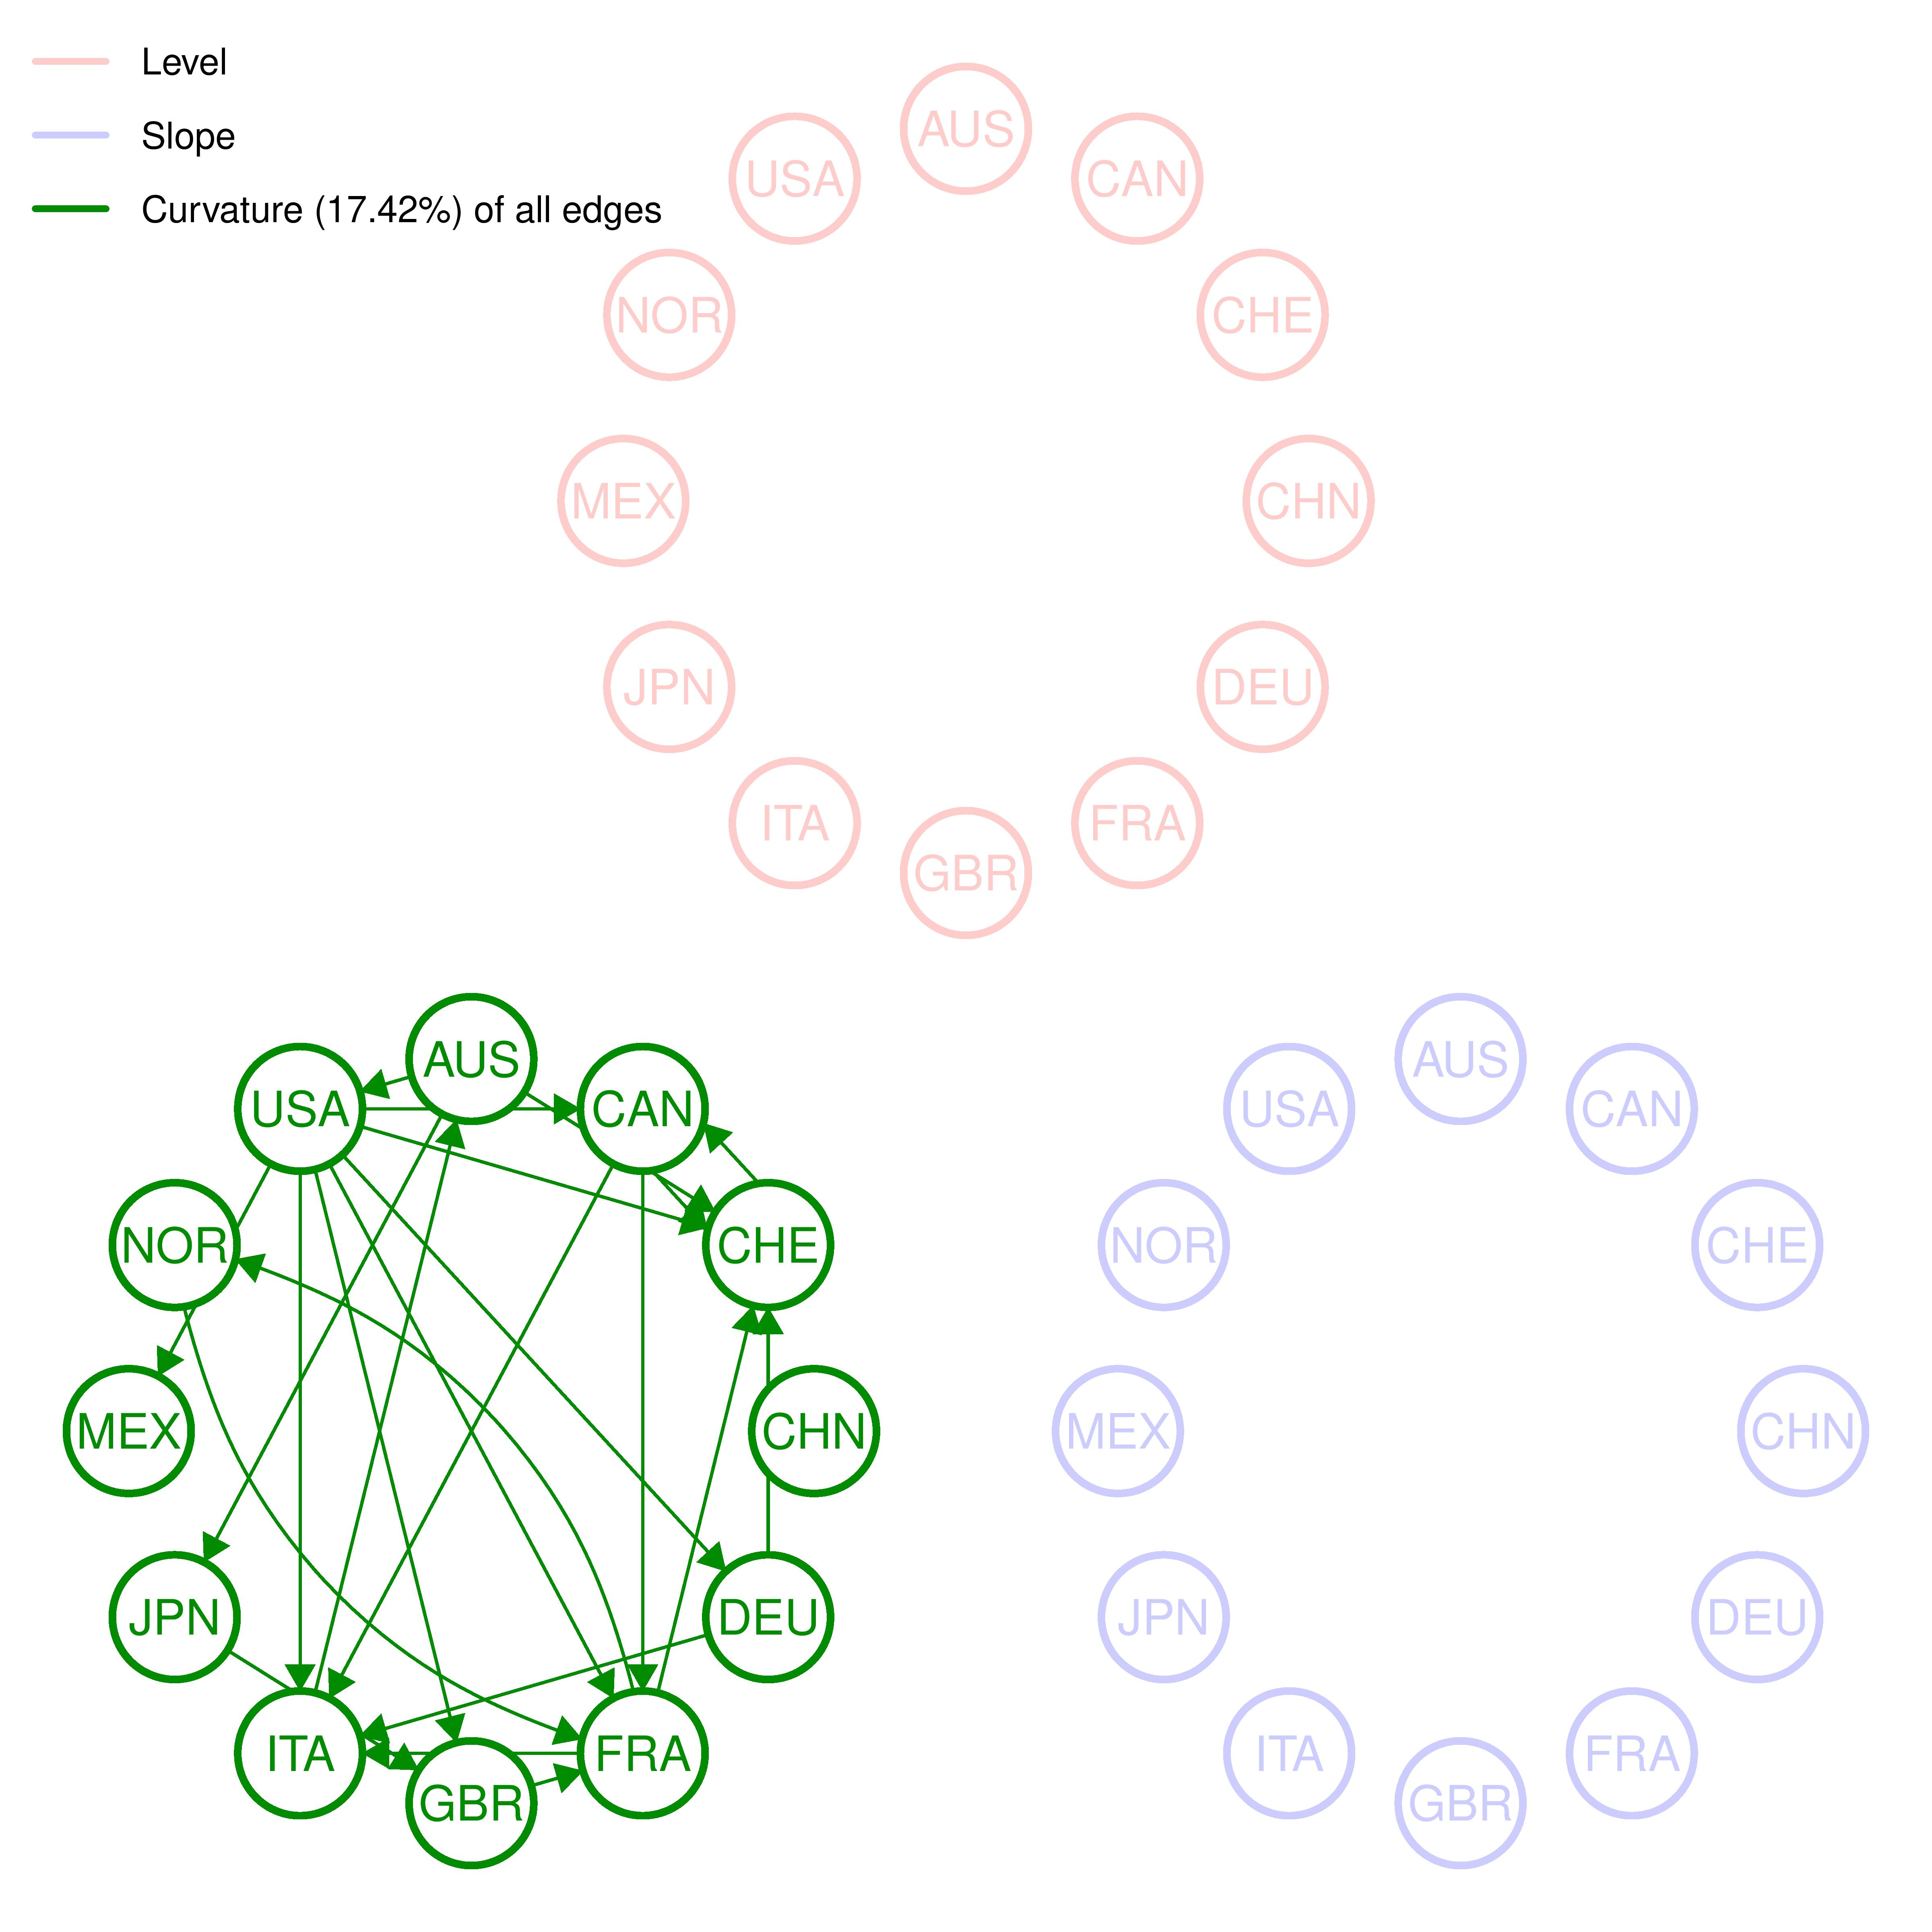
\includegraphics[width=\linewidth]{All_plot_onlycurv_2004-07-01_2019-12-31_0.01-page-001}
    \caption{\textbf{Curvatues only}: $A \setminus B$: Element liegt in $A$ \textbf{nicht} in $B$. (\textit{A ohne B})}
  \end{subfigure}
  \hfill
  \begin{subfigure}[t]{.4\textwidth}
    \centering
    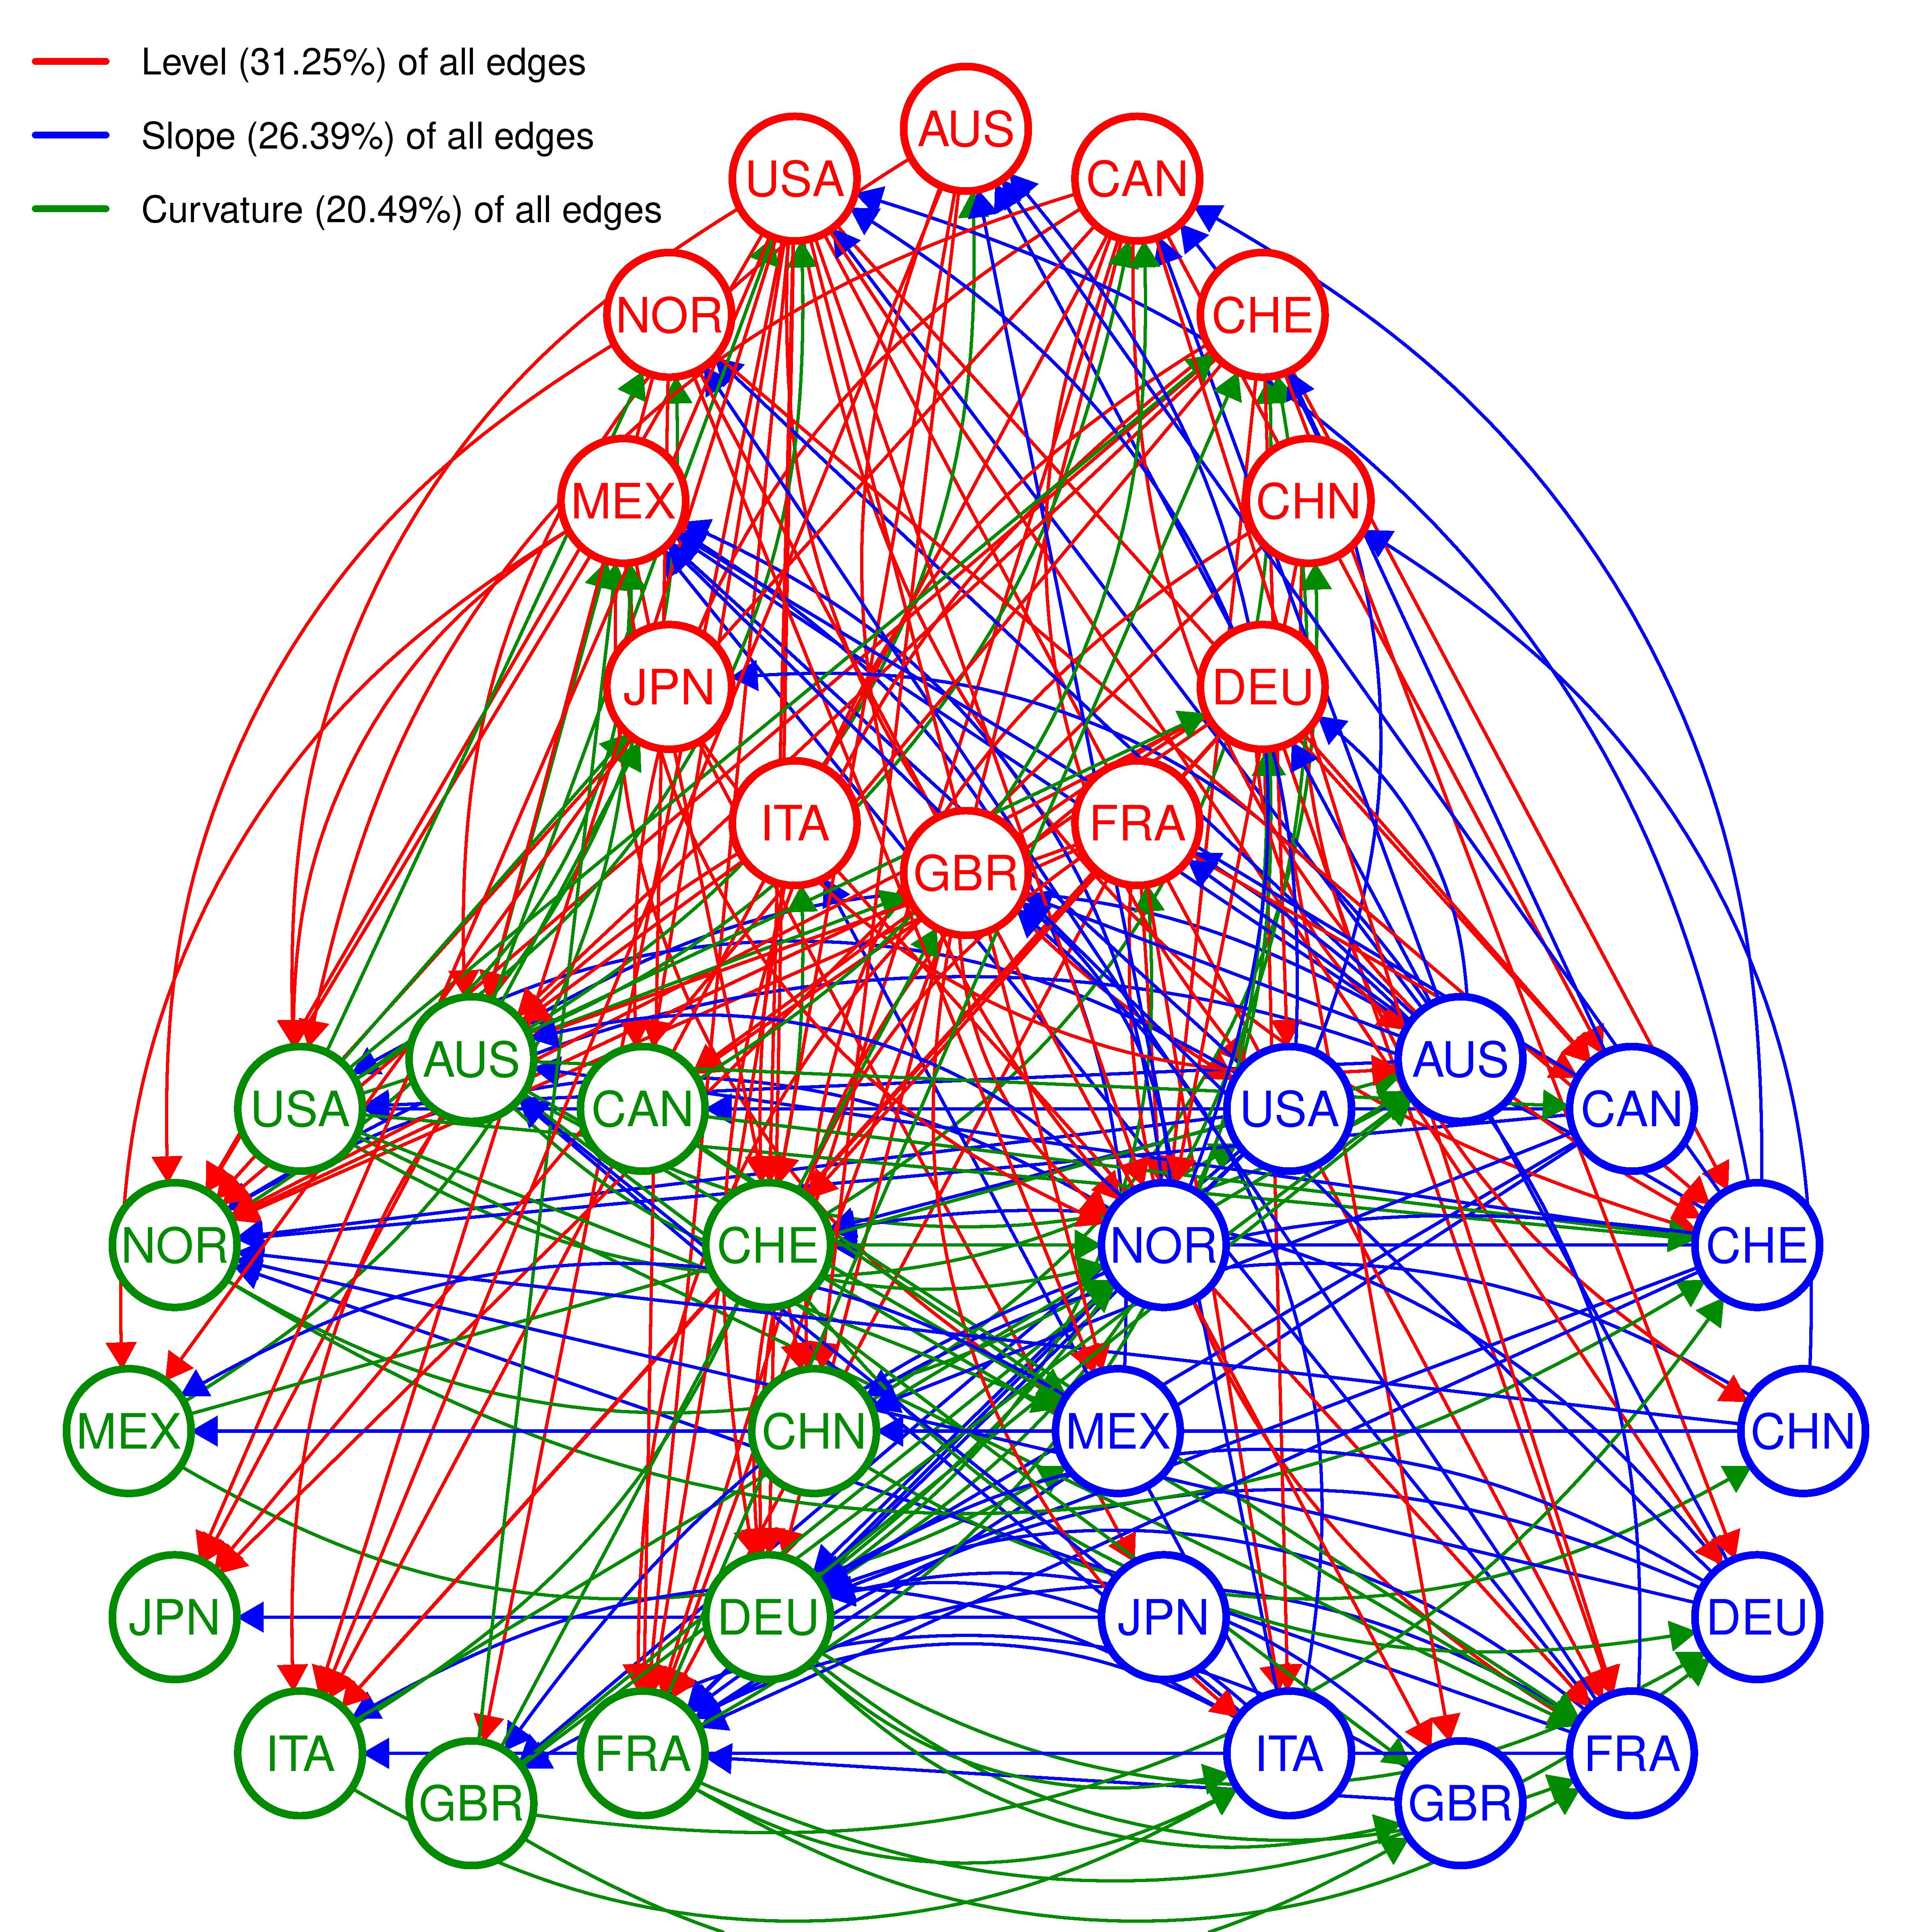
\includegraphics[width=\linewidth]{All_plot_innerempty_2004-07-01_2019-12-31_0.01-page-001}
    \caption{\textbf{Cross section only}: $A \Delta B$: Element liegt \textbf{entweder} in $A$ oder in $B$.}
  \end{subfigure}
\end{figure}



%----------------------------------------------------------------------------------------------------------------------------------------------------

\begin{table}[h]
\caption{Edge counts} %title of the table
\fontsize{10}{10}\selectfont
\centering% centering table
\begin{tabular}{l | ccc  r}% creating eight columns
\hline\hline \\ [-1.5ex]                         %inserting double-line

	&	Level	&	Slope	&	Curvature	& All  \\ 
\hline \\ [-1.5ex]  
Level	&	29	&	38	&	52	&	119 	\\
Slope	&	30	&	41	&	46	&	117	\\
Curvature	&	25	&	34	&	23	&	82	\\
\hline \\ [-1.5ex]  
All	&	84	&	113	&	121	&	318	\\


\hline            
\end{tabular}
\label{table:nonlin}% is used to refer this table in the text
\end{table}

%----------------------------------------------------------------------------------------------------------------------------------------------------

\begin{table}[h]
\caption{Edge ratio} %title of the table
\fontsize{10}{10}\selectfont
\centering% centering table
\begin{tabular}{l | ccc  r}% creating eight columns
\hline\hline \\ [-1.5ex]                         %inserting double-line


	&	Level	&	Slope	&	Curvature	&	All	\\
\hline \\ [-1.5ex] 
Level	&	21.970\%	&	26.389\%	&	36.111\%	&	84.470\%	\\
Slope	&	20.833\%	&	31.061\%	&	31.944\%	&	83.838\%	\\
Curvature	&	17.361\%	&	23.611\%	&	17.424\%	&	58.396\%	\\
\hline \\ [-1.5ex]  
All	&	60.164\%	&	81.061\%	&	85.480\%	&	25.238\%	\\


\hline            
\end{tabular}
\label{table:nonlin}% is used to refer this table in the text
\end{table}

%----------------------------------------------------------------------------------------------------------------------------------------------------

\begin{table}[h]
\caption{top nodes} %title of the table
\fontsize{10}{10}\selectfont
\setlength{\tabcolsep}{12pt}
\centering% centering table
\begin{tabular}{l  lcc  lc lc  lc}% creating eight columns

\hline\hline \\ [-1.5ex]                         %inserting double-line


\multicolumn{4}{c}{Top 5 all}					&	\multicolumn{2}{c}{Top 5 in}			&	\multicolumn{2}{c}{Top 5 out}			&	\multicolumn{2}{c}{Top 5 net}	\\	
\hline \\ [-1.5ex]    
Node	&	All	&	In	&	Out	&	Node	&	In	&	Node	&	Out	&	Node	&	Net	\\
\hline \\ [-1.5ex]    
USA\_L&	30	&	7	&	23	&	FRA\_C	&	19	&	USA\_L	&	23	&	USA\_L	&	16	\\
AUS\_S	&	28	&	11	&	17	&	NOR\_S	&	16	&	USA\_S	&	18	&	USA\_S	&	12	\\
FRA\_S	&	28	&	14	&	14	&	NOR\_C	&	16	&	USA\_C	&	17	&	USA\_C	&	10	\\
NOR\_S	&	27	&	16	&	11	&	MEX\_L	&	14	&	AUS\_S	&	17	&	DEU\_L	&	9	\\
FRA\_C	&	27	&	19	&	8	&	FRA\_S	&	14	&	DEU\_L	&	16	&	CAN\_L	&	7	\\

\hline            
\end{tabular}
\label{table:nonlin}% is used to refer this table in the text
\end{table}




\begin{figure}[H]
\caption{Node with most edges}
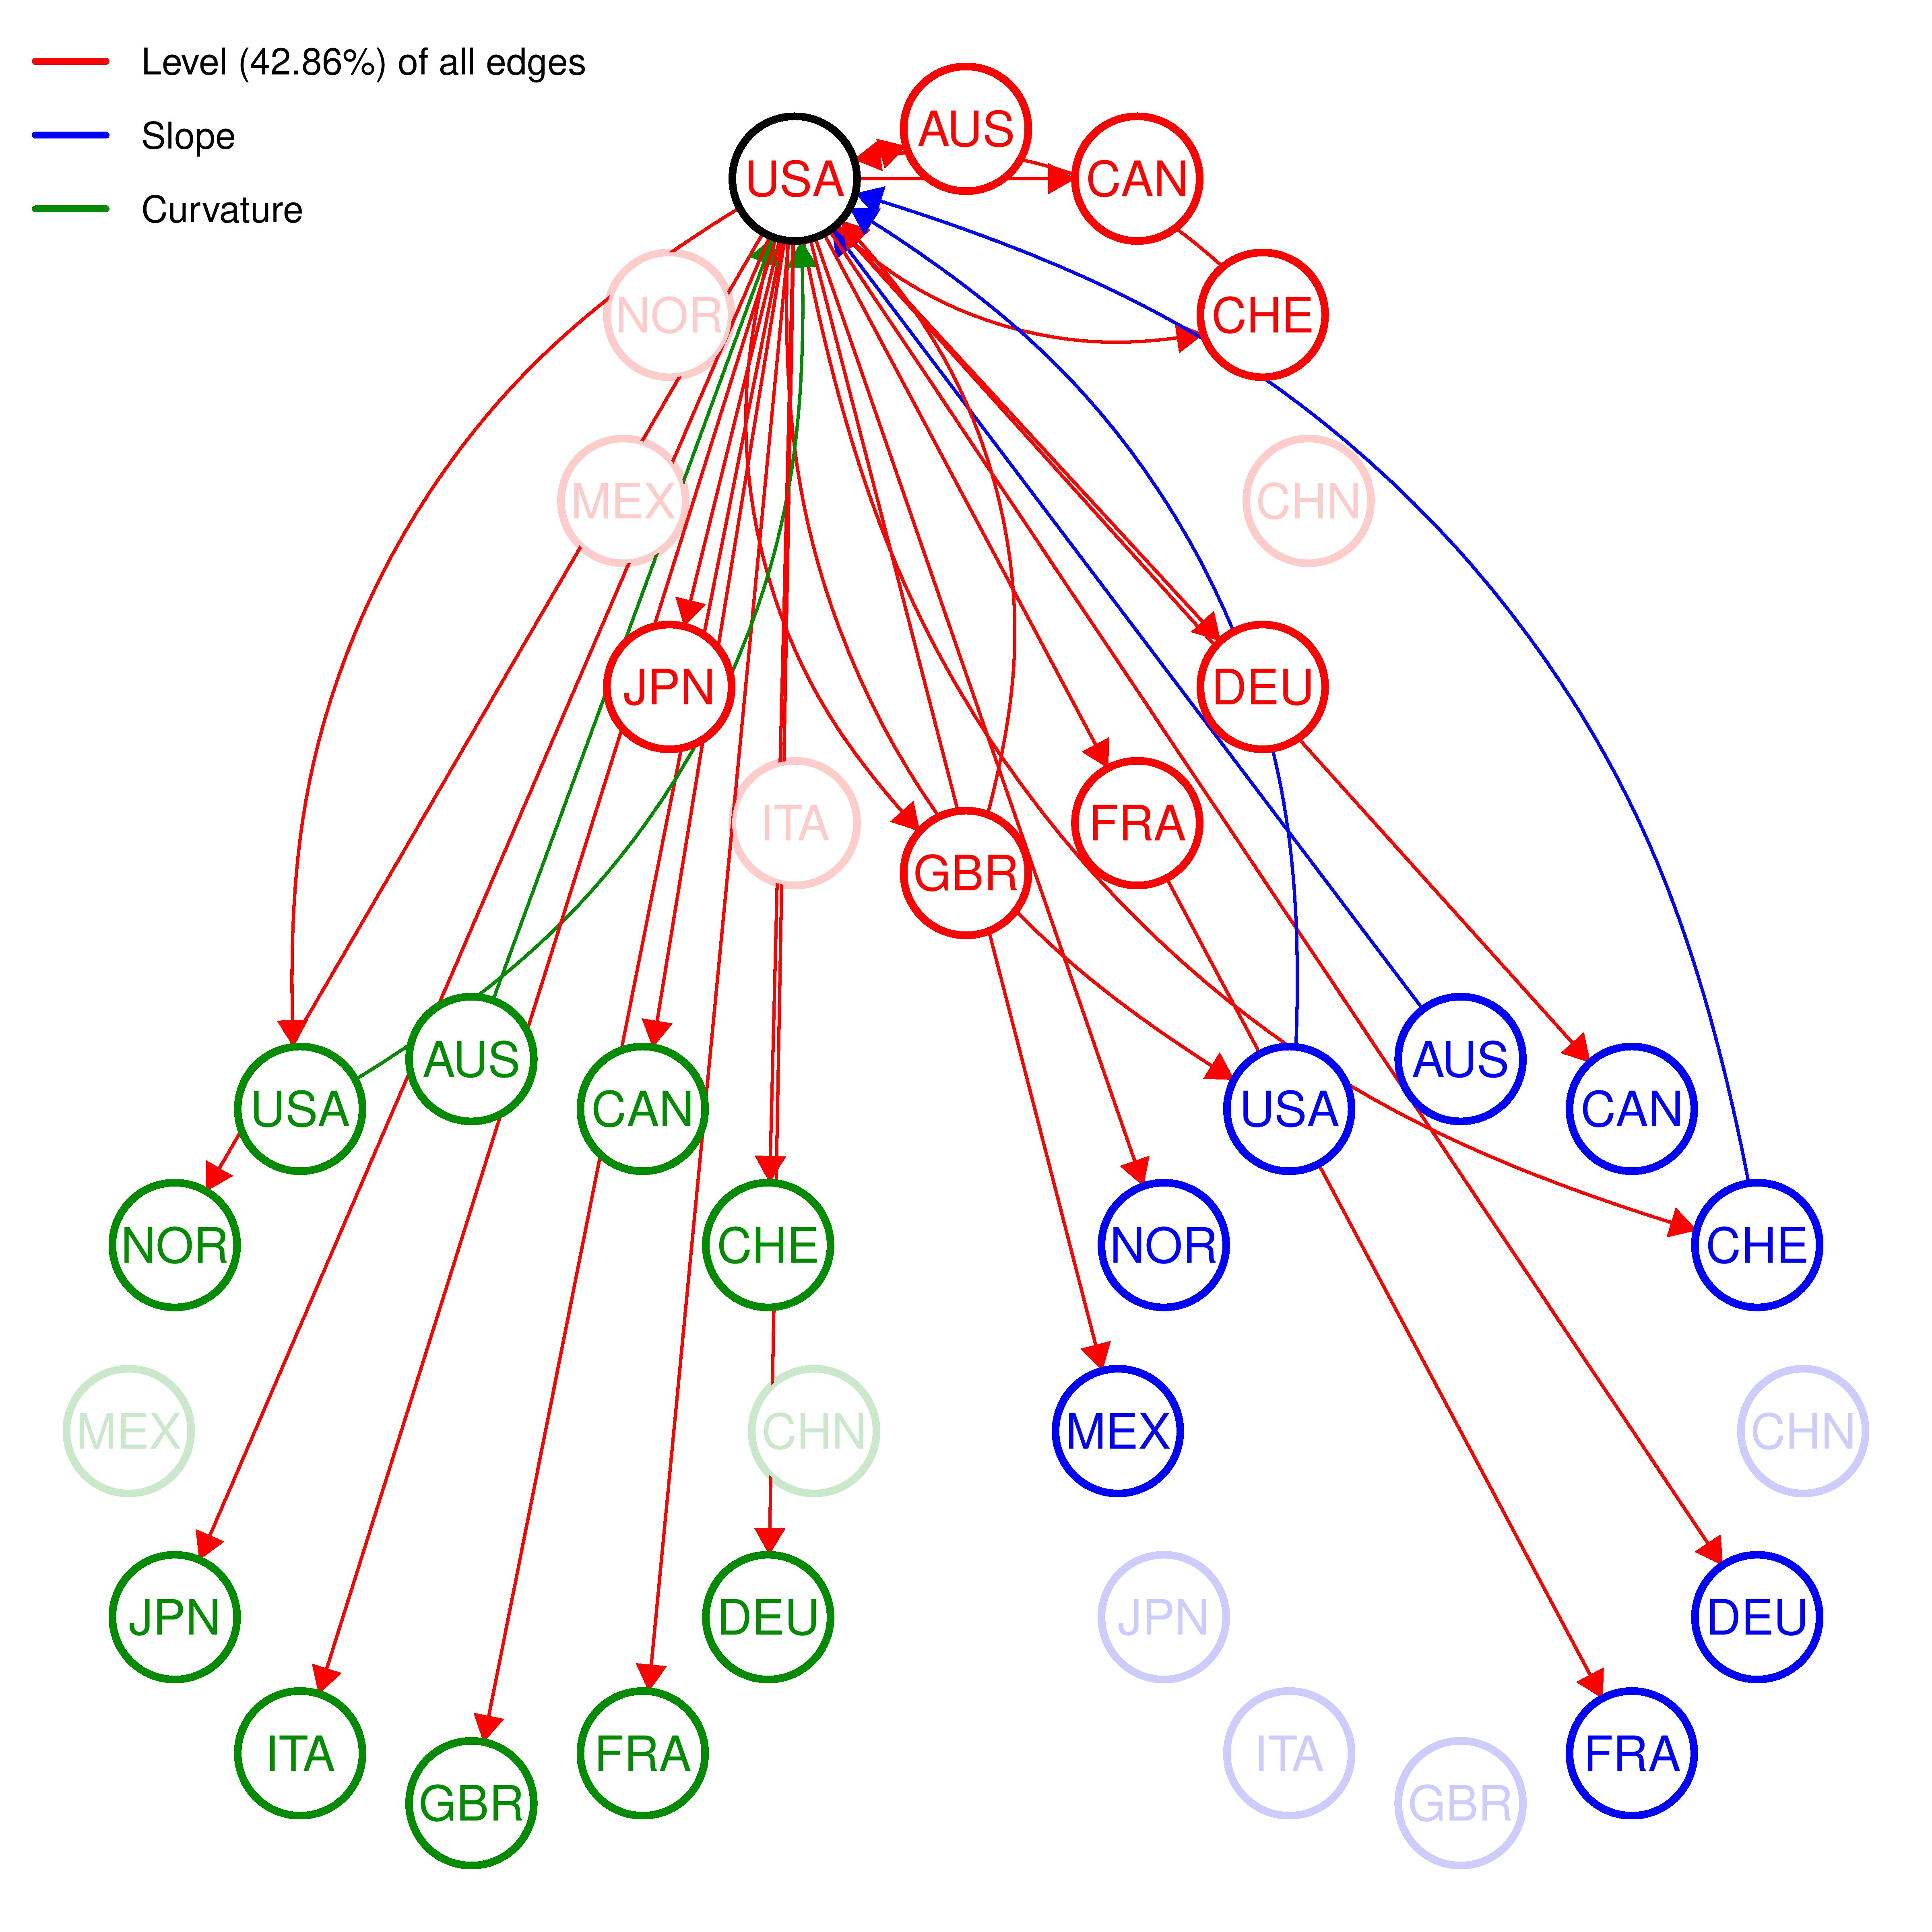
\includegraphics[width=11.5cm]{USA_B_1_plot_2004-07-01_2019-12-31_0.01-page-001}
\centering
\end{figure}



\begin{table}[h]
\caption{Daily TY} %title of the table
\fontsize{10}{10}\selectfont
\centering% centering table
\begin{tabular}{l | cccccc}% creating eight columns
\hline\hline \\ [-1.5ex]                         %inserting double-line


		& 	Whole &	First	&	Crisis I.& 	Second& 	Crisis II.&	 Third \\
\hline \\ [-1.5ex]  
Level	&		29	&	7	&	16.2	&	13.4	&  	12.1	&	 12\\
Slope	&		41	&	6	&	25.5	&	22.5	& 	16.2	& 	8.6\\
Curvature	&	23	&	7.3	&	20.7	&	9.7	& 	9.2	&	 9.9\\
Cross	&		225	&	61.8	&	142.2	&	109.1	& 	101.2	& 	76.1\\


\hline            
\end{tabular}
\label{table:nonlin}% is used to refer this table in the text
\end{table}

\begin{figure}[H]
\caption{750 window}
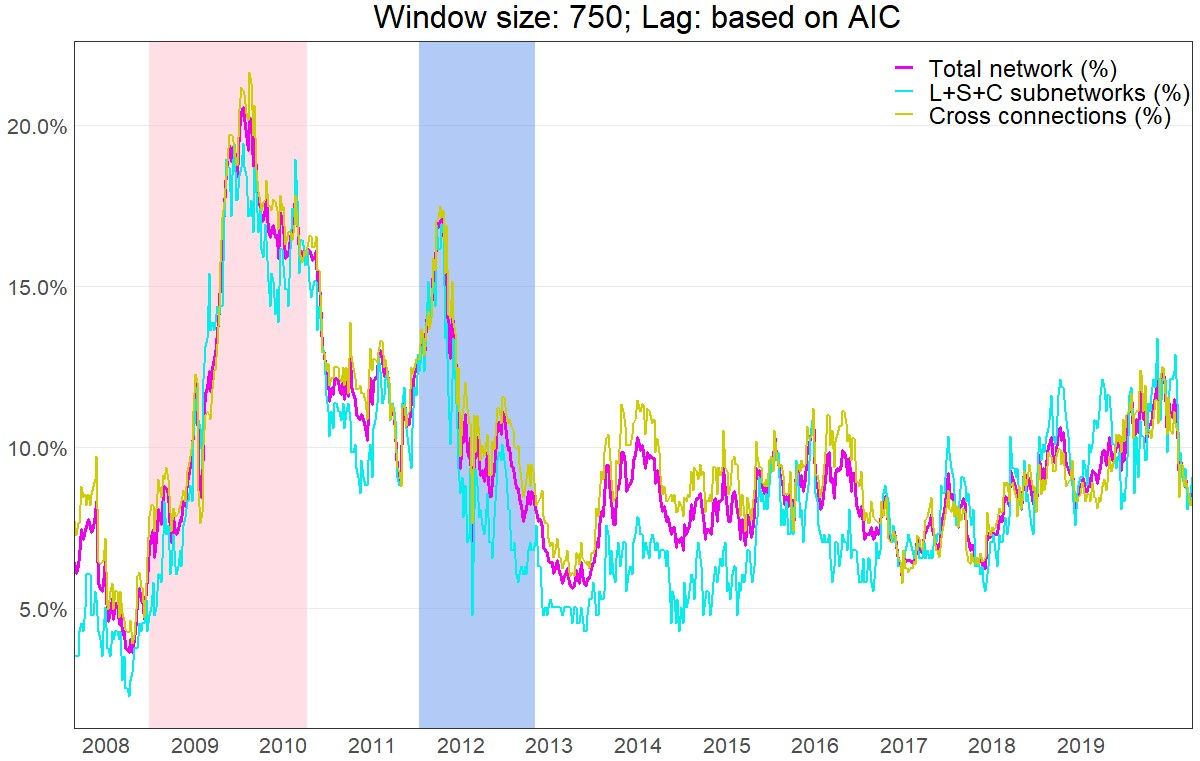
\includegraphics[width=11.5cm]{Time_series_750}
\centering
\end{figure}

\begin{figure}[H]
\caption{750 window}
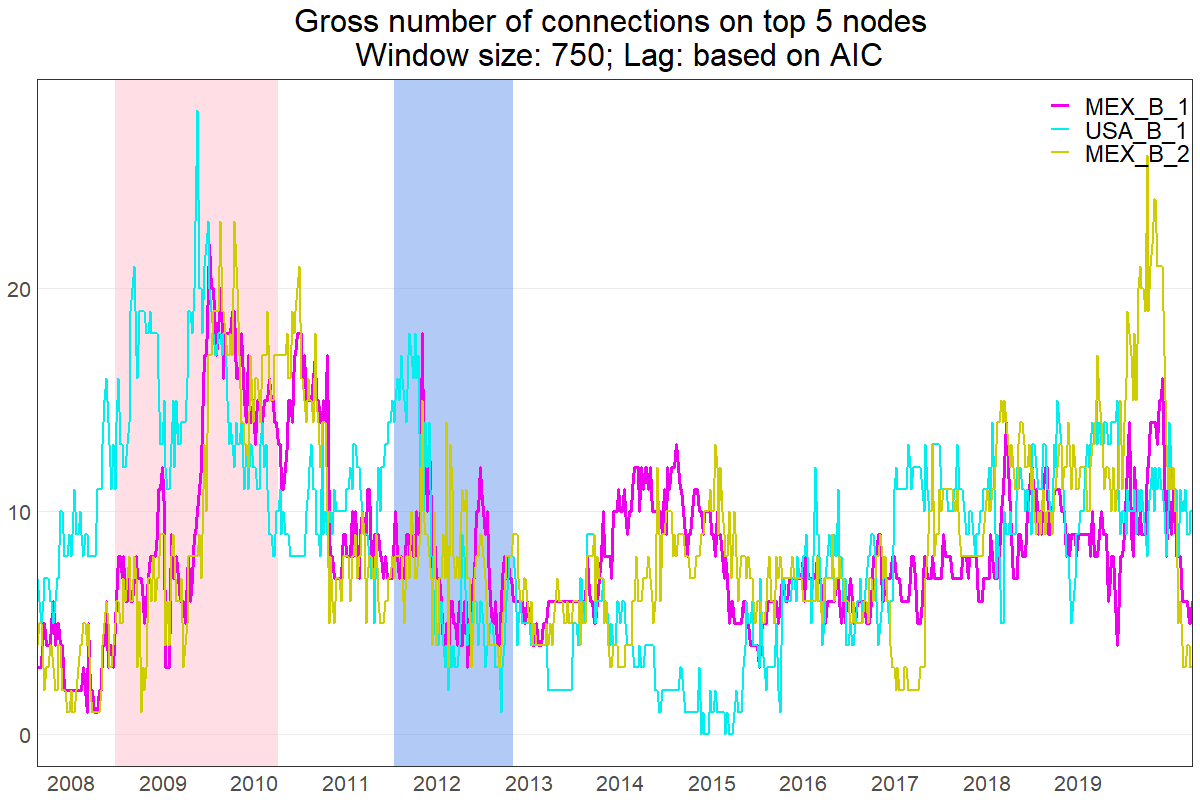
\includegraphics[width=11.5cm]{top5nodes}
\centering
\end{figure}

\begin{figure}[H]
\caption{500 / 1000 window}
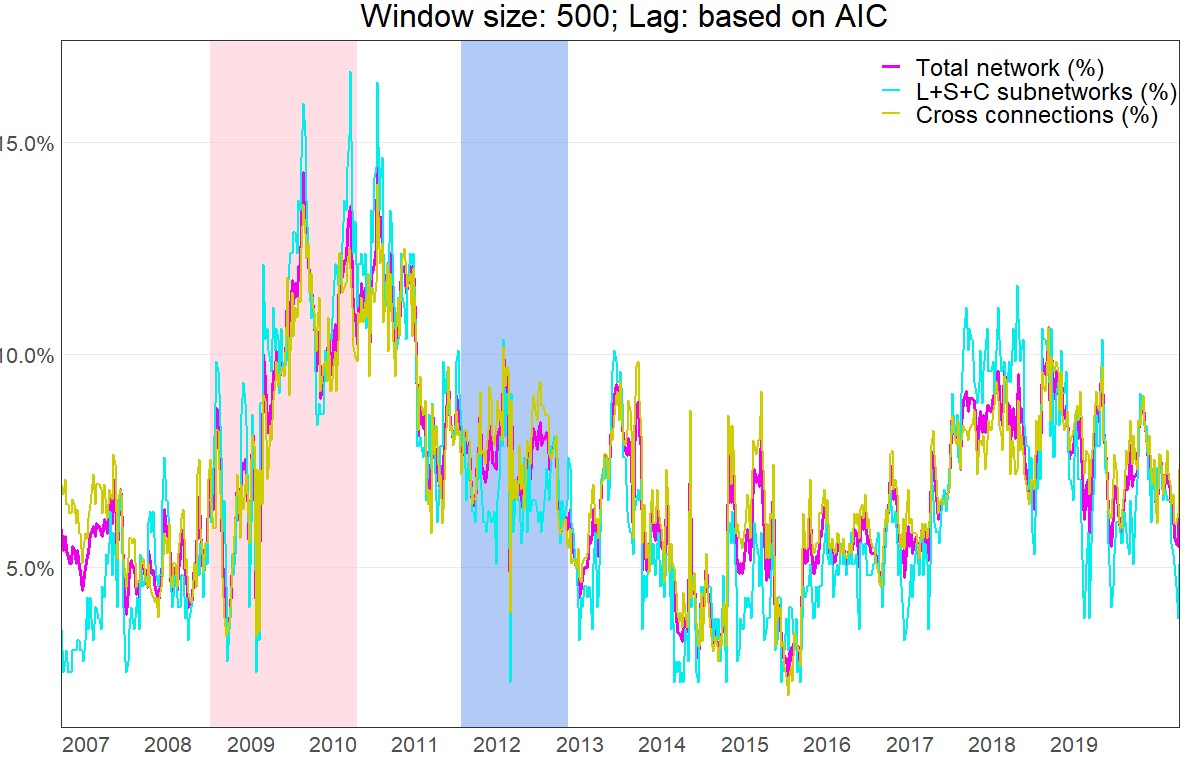
\includegraphics[width=11.5cm]{Time_series_500}
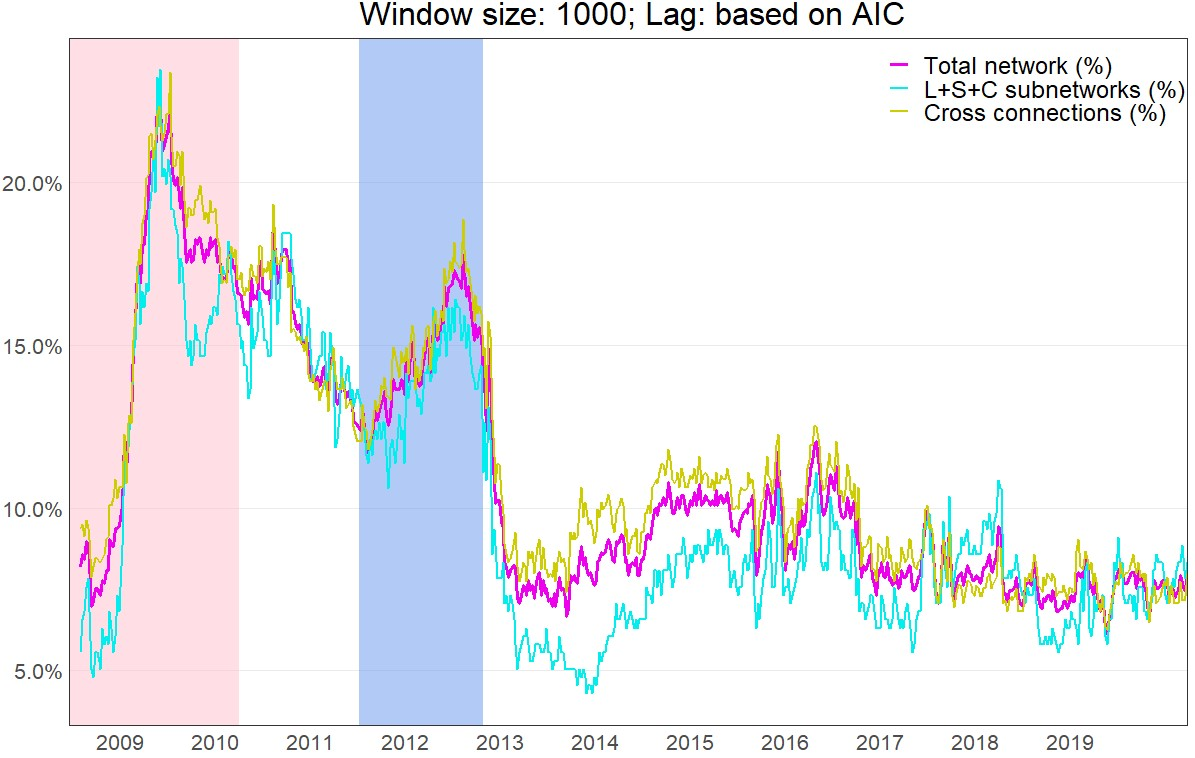
\includegraphics[width=11.5cm]{Time_series_1000}
\centering
\end{figure}



\section{Results}

This is a placeholder for results text

\bibliographystyle{te}

\FloatBarrier

\bibliography{research}[H]

\section{appendix}

\begin{table}[H]
\caption{This is the eaxemple table}% title of Table
\fontsize{10}{10}\selectfont
\centering % used for centering table
\begin{tabular}{l c c c c c c}% centered columns (4 columns)
\hline\hline   \\ [-1.5ex]               %inserts double horizontal lines
%Case & Method\#1 & Method\#2 & Method\#3 & test \\  [0.5ex]
Maturity & Mean & Std. Dev & Minimum & Maximum & \textrho(1)  & \textrho(10) \\ [0.5ex] % inserts table %heading

\hline       \\ [-1.5ex]           % inserts single horizontal line
\textit{Germany} 	&		&		&		&		&		&	\\
1 year	&	0.0256	&	1.6275	&	-0.9690	&	4.6900	&	1.0000	&	0.9960	\\
5 years	&	0.0257	&	1.6324	&	-0.9410	&	4.7670	&	0.9990	&	0.9930	\\
10 years	&	0.0243	&	1.5451	&	-0.7220	&	4.6860	&	0.9930	&	0.9640	\\
\medskip													
30 years	&	0.0228	&	1.4482	&	-0.2440	&	5.1950	&	0.9990	&	0.9880	\\
\textit{Italy}	&		&		&		&		&		&		\\
1 year	&	0.0241	&	1.5327	&	-0.4840	&	8.3940	&	0.9980	&	0.9860	\\
5 years	&	0.0239	&	1.5199	&	0.2370	&	7.8950	&	0.9980	&	0.9850	\\
10 years	&	0.0218	&	1.3876	&	0.8750	&	7.4920	&	0.9980	&	0.9860	\\
\medskip													
30 years	&	0.0188	&	1.1971	&	2.0430	&	7.5840	&	0.9980	&	0.9850	\\
\textit{France}	&		&		&		&		&		&		\\
1 year	&	0.0250	&	1.5891	&	-0.8010	&	4.6570	&	1.0000	&	0.9960	\\
5 years	&	0.0247	&	1.5730	&	-0.7730	&	4.9100	&	0.9990	&	0.9930	\\
10 years	&	0.0231	&	1.4670	&	-0.4150	&	4.8510	&	0.9990	&	0.9910	\\
\medskip													
30 years	&	0.0194	&	1.2351	&	0.4190	&	5.1160	&	0.9990	&	0.9860	\\
\textit{USA}	&		&		&		&		&		&		\\
1 year	&	0.0254	&	1.6128	&	0.0540	&	5.3230	&	1.0000	&	0.9980	\\
5 years	&	0.0194	&	1.2315	&	0.5590	&	5.3010	&	0.9990	&	0.9890	\\
10 years	&	0.0163	&	1.0394	&	1.3890	&	5.3880	&	0.9980	&	0.9830	\\
30 years	&	0.0151	&	0.9618	&	1.9920	&	5.8390	&	0.9970	&	0.9760	\\
\textit{Canada}	&		&		&		&		&		&		\\
1 year	&	0.0193	&	1.2301	&	0.3000	&	4.8090	&	1.0000	&	0.9950	\\
5 years	&	0.0180	&	1.1463	&	0.4840	&	4.8010	&	0.9990	&	0.9890	\\
10 years	&	0.0173	&	1.0976	&	0.9830	&	5.0760	&	0.9990	&	0.9870	\\
\medskip													
30 years	&	0.0159	&	1.0118	&	1.3060	&	5.6120	&	0.9980	&	0.9850	\\
\textit{Mexico}	&		&		&		&		&		&		\\
1 year	&	0.0318	&	2.0250	&	1.5120	&	10.5700	&	0.9790	&	0.9880	\\
5 years	&	0.0238	&	1.5108	&	3.7860	&	10.8970	&	0.9860	&	0.9810	\\
10 years	&	0.0213	&	1.3524	&	4.6190	&	12.4130	&	0.9920	&	0.9700	\\
30 years	&	0.0195	&	1.2384	&	5.8730	&	12.7260	&	0.9930	&	0.9470	\\
\textit{Japan}	&		&		&		&		&		&		\\
1 year	&	0.0043	&	0.2715	&	-0.3710	&	0.8500	&	0.9990	&	0.9920	\\
5 years	&	0.0076	&	0.4852	&	-0.3960	&	1.6310	&	0.9990	&	0.9900	\\
10 years	&	0.0103	&	0.6563	&	-0.2850	&	2.0500	&	0.9990	&	0.9900	\\
\medskip													
30 years	&	0.0120	&	0.7606	&	0.0530	&	3.2950	&	0.9980	&	0.9850	\\
\textit{China}	&		&		&		&		&		&		\\
1 year	&	0.0115	&	0.7296	&	0.9570	&	4.3820	&	0.9920	&	0.9660	\\
5 years	&	0.0093	&	0.5939	&	1.7820	&	4.8740	&	0.9970	&	0.9730	\\
10 years	&	0.0090	&	0.5702	&	2.4810	&	5.5030	&	0.9930	&	0.9640	\\
\medskip													
30 years	&	0.0097	&	0.6149	&	2.4700	&	6.0090	&		&		\\
\textit{Australia}	&		&		&		&		&		&		\\
1 year	&	0.0279	&	1.7749	&	0.6750	&	7.3760	&	0.9990	&	0.9920	\\
5 years	&	0.0264	&	1.6769	&	0.6390	&	6.9600	&	0.9990	&	0.9900	\\
10 years	&	0.0235	&	1.4971	&	0.8850	&	6.8730	&	0.9990	&	0.9880	\\
\medskip													
30 years	&	0.0190	&	1.2069	&	1.5580	&	6.8880	&	0.9980	&	0.9830	\\
\textit{Norway}	&		&		&		&		&		&		\\
1 year	&	0.0222	&	1.4100	&	0.1990	&	6.2430	&	0.9990	&	0.9940	\\
5 years	&	0.0200	&	1.2734	&	0.5450	&	5.3350	&	0.9990	&	0.9910	\\
10 years	&	0.0188	&	1.1935	&	0.8880	&	5.2760	&	0.9990	&	0.9890	\\
\medskip													
30 years	&	0.0175	&	1.1127	&	0.8820	&	5.2730	&	0.9990	&	0.9870	\\
\textit{United Kingdom}	&		&		&		&		&		&		\\
1 year	&	0.0308	&	1.9558	&	0.0240	&	5.8830	&	0.9990	&	0.9950	\\
5 years	&	0.0259	&	1.6444	&	0.1610	&	5.8210	&	0.9990	&	0.9910	\\
10 years	&	0.0223	&	1.4181	&	0.4000	&	5.5430	&	0.9990	&	0.9890	\\
\medskip													
30 years	&	0.0175	&	1.1099	&	0.9390	&	5.0700	&	0.9990	&	0.9870	\\
\textit{Switzerland}	&		&		&		&		&		&		\\
1 year	&	0.0195	&	1.2405	&	-1.1650	&	3.3750	&	1.0000	&	0.9960	\\
5 years	&	0.0187	&	1.1921	&	-1.1960	&	3.2000	&	0.9990	&	0.9930	\\
10 years	&	0.0188	&	1.1976	&	-1.1380	&	3.4550	&	0.9990	&	0.9910	\\
30 years	&	0.0173	&	1.1006	&	-0.6440	&	3.7330	&	0.9980	&	0.9860	\\

\hline%inserts single line
\end{tabular}
\label{table:nonlin}% is used to refer this table in the text
\end{table}

\end{document}

